\documentclass[a4paper,12pt,UTF8]{ctexart}

% if you need to pass options to natbib, use, e.g.:
\PassOptionsToPackage{numbers, compress}{natbib}
% before loading nips_2016
%
% to avoid loading the natbib package, add option nonatbib:
% \usepackage[nonatbib]{nips_2016}

%\usepackage{nips_2016}

% to compile a camera-ready version, add the [final] option, e.g.:
\usepackage[final]{finalreport}

\usepackage[utf8]{inputenc} % allow utf-8 input
\usepackage[T1]{fontenc}    % use 8-bit T1 fonts
\usepackage{hyperref}       % hyperlinks
\usepackage{url}            % simple URL typesetting
\usepackage{booktabs}       % professional-quality tables
\usepackage{amsfonts}       % blackboard math symbols
\usepackage{nicefrac}       % compact symbols for 1/2, etc.
\usepackage{microtype}      % microtypography
\usepackage{CJKutf8}
\usepackage{graphicx}
\usepackage{float}
\usepackage{amsmath}
\usepackage{pdfpages}
\usepackage{titlesec}
\usepackage{indentfirst}

\setlength{\parindent}{2em}

\newcommand{\norm}[1]{\left\lVert#1\right\rVert}

\title{《人工神经网络》大作业最终报告:神经图像编辑}


% The \author macro works with any number of authors. There are two
% commands used to separate the names and addresses of multiple
% authors: \And and \AND.
%
% Using \And between authors leaves it to LaTeX to determine where to
% break the lines. Using \AND forces a line break at that point. So,
% if LaTeX puts 3 of 4 authors names on the first line, and the last
% on the second line, try using \AND instead of \And before the third
% author name.

\newcommand{\song}{\CJKfamily{zhsong}}	% 宋体
\newcommand{\hei}{\CJKfamily{zhhei}}	% 黑体
\newcommand{\fs}{\CJKfamily{zhfs}}		% 仿宋
\newcommand{\kai}{\CJKfamily{zhkai}}	% 楷体
\newcommand{\li}{\CJKfamily{zhli}}		% 隶书
\newcommand{\you}{\CJKfamily{zhyou}}	% 幼圆

\author{
  徐鉴劲 \\
  2015011313 \\
  计算机科学与技术系 \\
  清华大学 \\
  \texttt{xujj15@mails.tsinghua.edu.cn}
  %% examples of more authors
  \AND
  贾越凯 \\
  2015011335 \\
  计算机科学与技术系 \\
  清华大学 \\
  \texttt{jiayk15@mails.tsinghua.edu.cn} \\
  \AND
  寇明阳 \\
  2015011318 \\
  计算机科学与技术系 \\
  清华大学 \\
  \texttt{kmy15@mails.tsinghua.edu.cn} \\
  %% \And
  %% Coauthor \\
  %% Affiliation \\
  %% Address \\
  %% \texttt{email} \\
}

\begin{document}

\maketitle

\begin{abstract}

图像是人类重要的交互途径,然而大部分人却不具有绘画的才能。本项目中,编辑的方法成功地应用在了动漫人脸生成的领域,用户只用给出简笔画就可以对图像进行符合人类直觉的变换,对人物的发色、瞳色、发型进行自由度极高的编辑操作。目前有关机器图像编辑的研究中普遍没有使用一个强大的生成器,以至于生成结果十分粗糙,在编辑不稳定而极易失去图像的真实性,也没有在动漫人脸领域的应用。我们使用了自行收集的Getchu动漫人脸数据集,结合Auxiliary Classifier GAN和DRAGAN成功地训练了复杂的生成器、判别器,并将编辑操作成功地应用在了训练好的模型上。对比基线方法,我们大幅提高了生成的质量与清晰度,提升了编辑的稳定性,并完成了一个与用户交互的Web前端。此外,我们进行了多种GAN训练方法的对比,在MNIST数据集上也进行了实验。

\end{abstract}


\section{引言}

图像是人类重要的交互途径,然而大部分人却不具有绘画的才能,本项目意图在于以人工智能的手段降低非专业人士在绘图方面的技术壁垒。在我们的作品神经图像编辑中,用户给出简笔画就可以得到算法生成的与预期相似的图画;用户还可以继续完善简笔画,对图像进行符合人类直觉的图像编辑,达到更符合预期的结果。
通过简笔画生成图像的技术有着广泛的应用前景,例如基于草图的商品搜索,适用于个体创作人的插图绘制,面向兴趣爱好者的辅助工具等等。

神经图像编辑的范围十分广阔,本项目研究动漫头像编辑这一子类上的应用。

经过一个学期的时间,我们的项目取得了如下成果:

\begin{enumerate}
\item 成功复现了高质量的动漫人物头像生成网络。
\item 成功应用编辑图像方法于极深层的神经网络。
\item 获得了高于基线的生成成果和编辑成果。包括生成真实度上升,生成清晰度上升($64 \times 64 \Rightarrow 128 \times 128$)和肉眼可见的编辑质量上升
\item 基于Web/Server的交互界面。
\end{enumerate}

\begin{figure}[H]
  \centering
  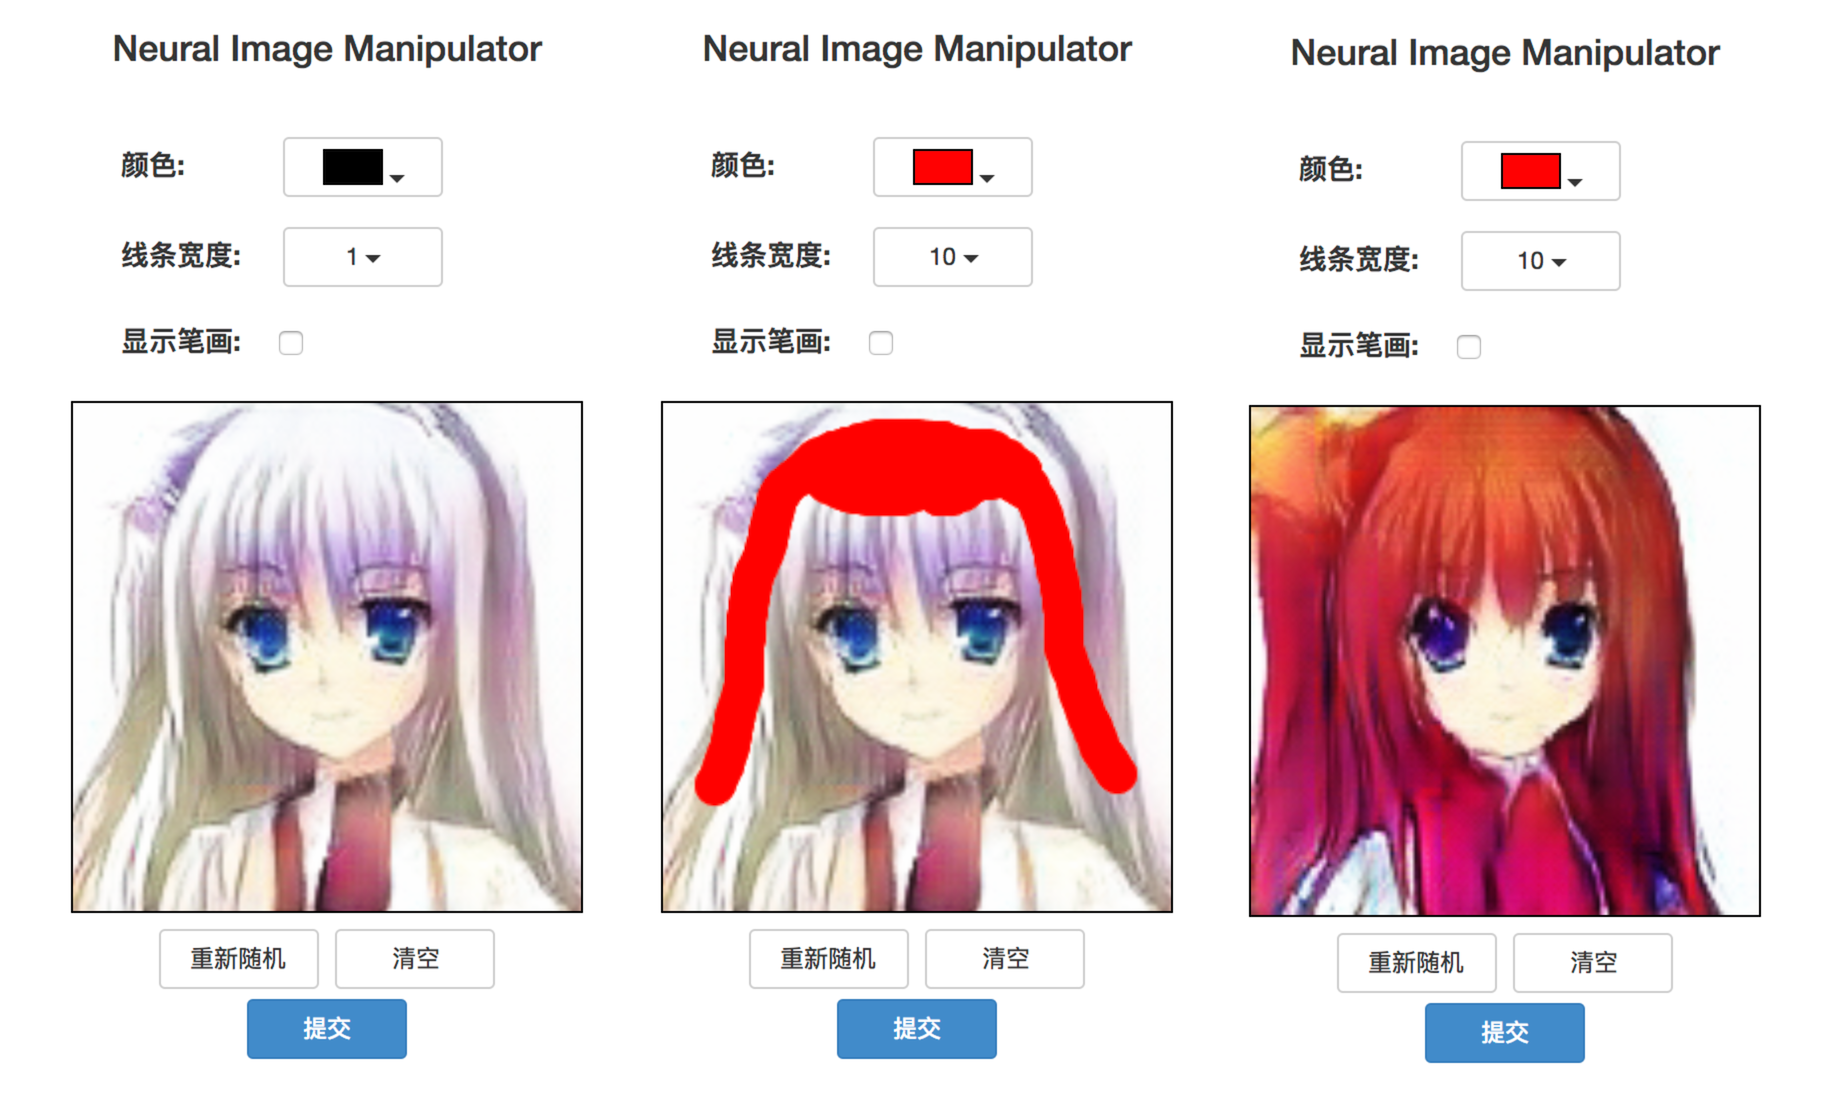
\includegraphics[width=0.9\linewidth]{figs/frontend.png}
  \caption{\kai 项目效果展示。用户通过网页前端绘制简笔画,提交到后台,经过神经网络的优化编辑以后,返回一个符合编辑预期的图像。}
  \label{fig:frontend}
\end{figure}


\section{相关工作}


现有的研究中,与草图生成图像相关的研究可以分为两类,一类是使用语义图像作为输入的条件生成网络,一类是将编辑过程看作可优化的过程,调整生成器的输入的方法。前一类以pix2pix为代表~\cite{isola2016image},输入一个精确的语义地图(semantic segmentation map),每一个像素表明了所属的物体类别,通过一个变化后的AutoEncoder输出生成图像。后一类使用普通的生成网络,接受随机向量的输入,输出生成图像,通过设计一种改变输入随机向量的方法来使得网络生成靠近期望结果的输出。

由于动漫人脸生成任务的约束,我们没有语义精确的数据集,难以按照原文复现第一类方法,所以不与之比较。本项目比较的baseline主要有两个,一个是交互式生成对抗网络iGAN~\cite{Zhu2016Generative},一个是神经图像编辑器Neural Photo Editor~\cite{Brock2016Neural}。这两个均可以完成编辑功能,然而他们的问题主要有:

\begin{enumerate}
\item 生成精度低。这两个工作并没有将编辑的操作应用在强大的生成网络上,生成的精度最高只能达到 $64 \times 64$。
\item 没有应用于动漫画风的领域上。这两个工作的数据集都是较为完善的真实数据集图片,如户外风景和人类图片数据集,然而本项目中涉及到的动漫数据集属于难度较高的类型,是从网络上爬取的数据集、规模较小、画风多样、混杂有低质量图片等等。
\item 编辑中有很大的可能丧失图片类别的特性,丧失人脸的特征。
\end{enumerate}

这些问题在下面的例子中都有体现,然而下面的例子已经是经过多次尝试而得到的最好结果。

\begin{figure}[H]
  \centering
  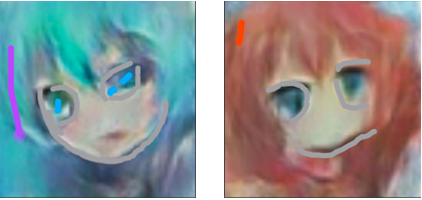
\includegraphics[width=0.9\linewidth]{figs/baseline1.PNG}
  \caption{\kai iGAN在收集到的Getchu数据集上的复现,使用iGAN开源的代码,遵循了原文的设置。图中灰色线条是边缘简笔画,其他的彩色线条是颜色简笔画,图片是在这些简笔画限制下的编辑结果。在生成的过程中经理了频繁的失败,极易丧失生成结果的真实行。展示的图片经过了精心挑选,达到了iGAN所能达到的最佳效果,然而结果仍然十分不美观。}
  \label{fig:baseline1}
\end{figure}

\begin{figure}[H]
  \centering
  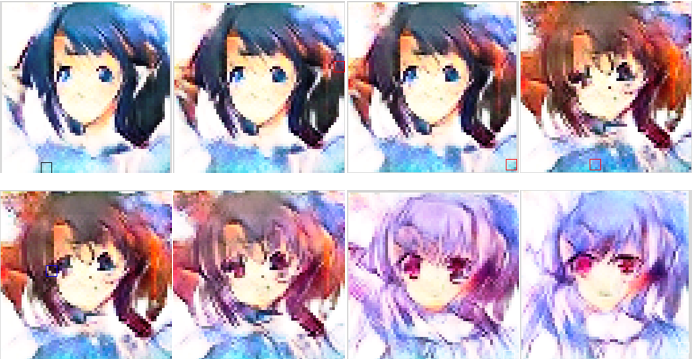
\includegraphics[width=0.9\linewidth]{figs/baseline2.PNG}
  \caption{\kai Neural Photo Editor (NPE) 在Getchu数据集上的复现,使用了NPE开源的代码,遵循了原文的设置。从左上到右下是在神经图像编辑过程中顺序产生的,用户在$1\sim5$张中头发的位置画了红色线条,并在 $6\sim8$张中画了蓝色线条。线条在图中没有显示出来,图中有时出现的小方框是画笔的光标,可以忽略。头像颜色变化基本与预期相符,体现了编辑的有效性。}
  \label{fig:baseline2}
\end{figure}

\section{方法}

\begin{figure}[H]
  \centering
  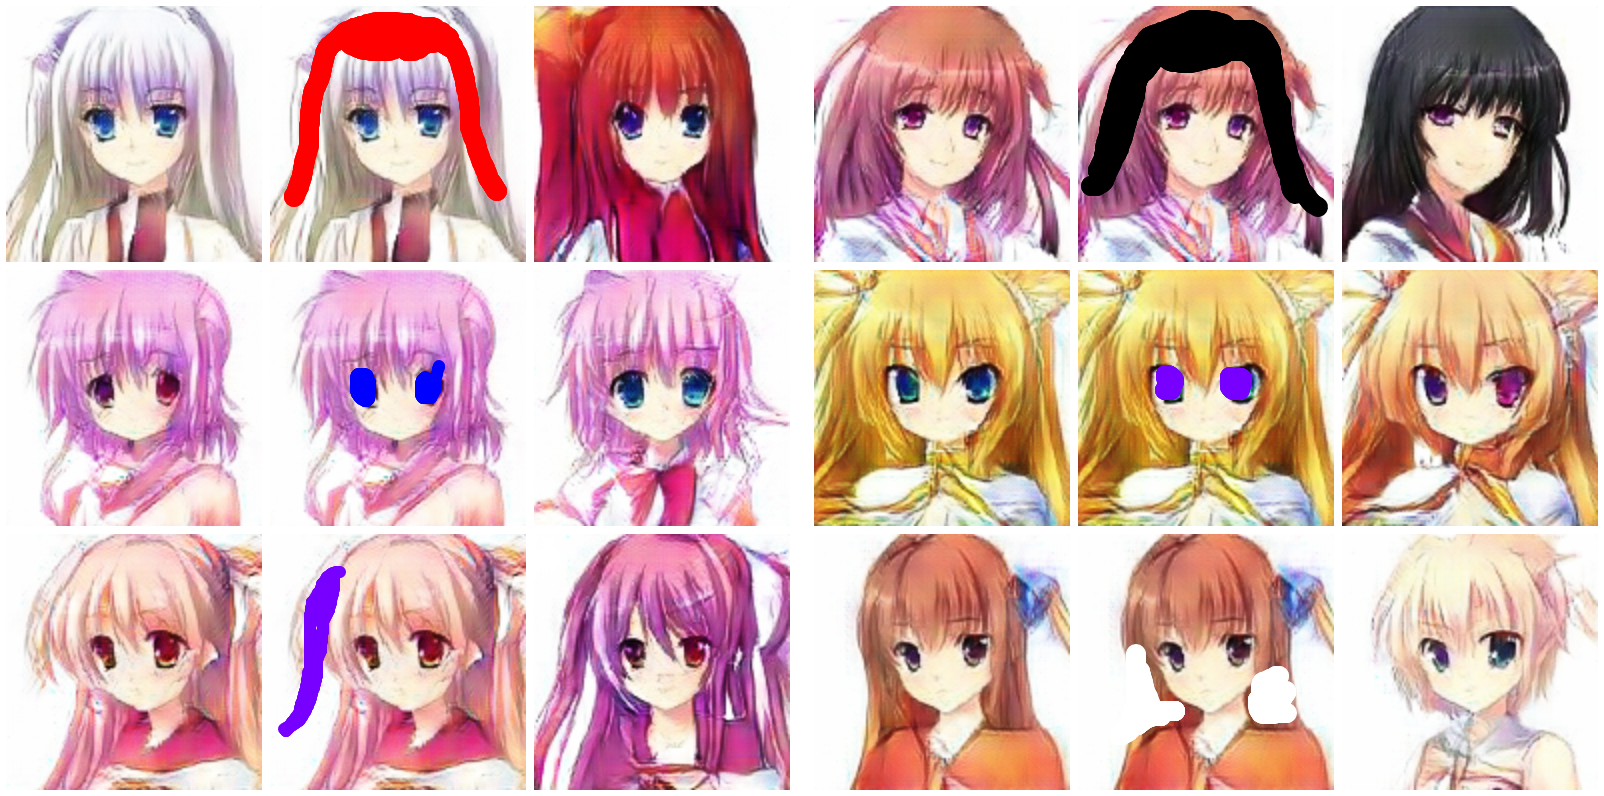
\includegraphics[width=0.9\linewidth]{figs/pic.png}
  \caption{\kai 编辑效果展示,共六组,每组三幅图。每组中最左边的一幅为原图,中间的一幅图为编辑图,最右边的一幅图为生成的结果图。第一行为成功更换发色的例子,第二行为成功更换瞳色的例子,第三行为成功更换发型的例子。}
  \label{fig:pic}
\end{figure}

\subsection{框架}

我们的项目分为两个阶段实现,第一阶段不编辑一个给定的具体图像,先考虑编辑一个随机生成的图像,如图 \ref{fig:workflow1};第二阶段再加入一个编码网络来完成对于具体图像的编辑,在图 \ref{fig:workflow2} 中进行了说明。目前我们已经完成了第一个阶段的工作,第二个阶段完成了网络的训练,正在进行前端的调整,以支持上传图像并编辑的功能。

\begin{figure}[H]
  \centering
  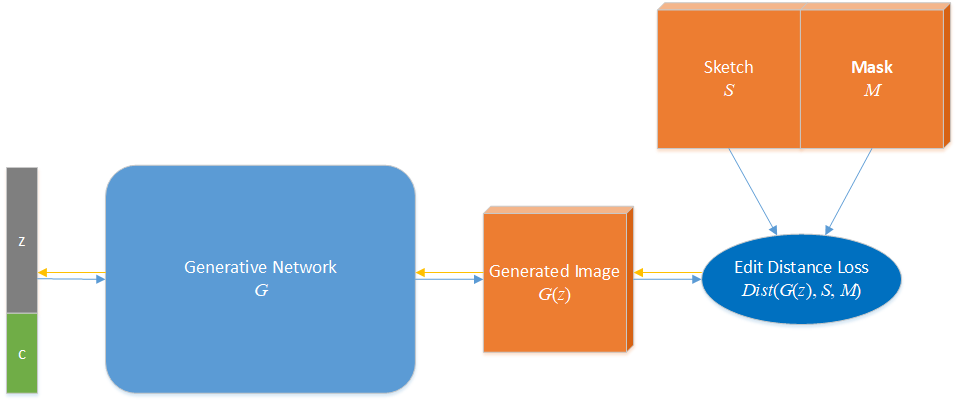
\includegraphics[width=1\linewidth]{figs/workflow1.png}
  \caption{\kai 第一阶段的项目解决方法。从随机向量出发,由生成网络生成初始结果,用户给定简笔画和对应的遮罩,由编辑距离函数计算误差和倒数,并借此更新 $z$,达到编辑图像的目的。蓝箭头表示数据流向,橙色箭头表示导数。}
  \label{fig:workflow1}
\end{figure}

\begin{figure}[H]
  \centering
  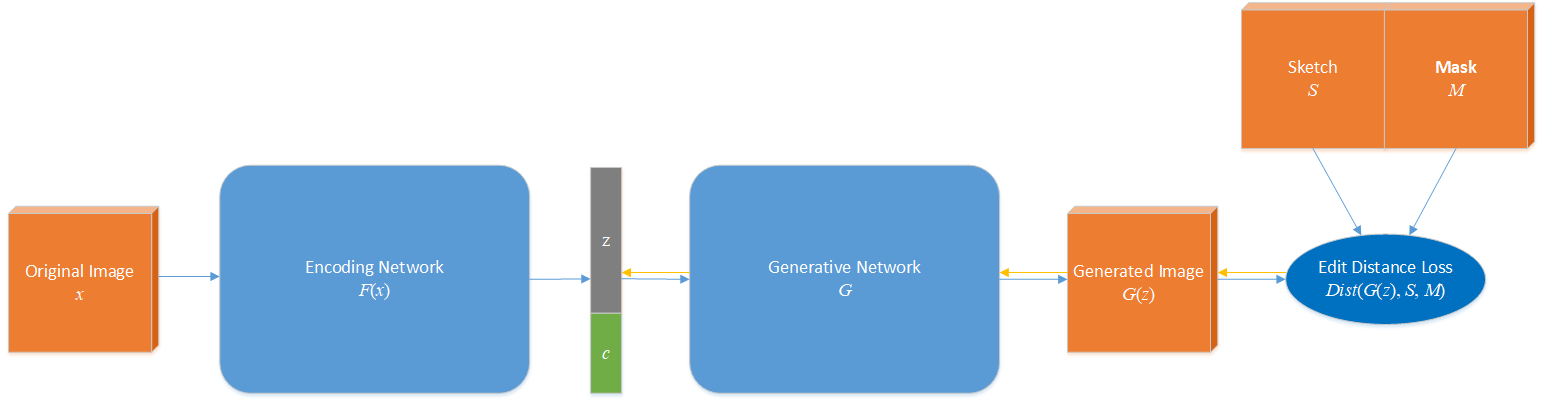
\includegraphics[width=1\linewidth]{figs/workflow2.png}
  \caption{\kai 第二阶段的项目解决方法。从一个待编辑图像出发,先通过编码网络生成 $z$ 与 $c$,然后经过生成网络生成重构结果,用户给定简笔画(sketch)和对应的遮罩(mask),由编辑距离函数计算误差和导数,并借此更新 $z$,达到编辑图像的目的。蓝箭头表示数据流向,橙色箭头表示导数。}
  \label{fig:workflow2}
\end{figure}

\subsection{编辑图像}

我们使用训练好的生成网络$G$实现对于图像的编辑工作。

一个生成网络$G(z, c)$接受随机向量$z$(遵循高斯分布)和条件向量$c$作为输入,生成图像$I = G(z, c)$。同时用户给定编辑图像$I'$,例如一副简笔画,则可以据此给出生成图像与编辑图像之间的距离$Dist(G(z, c), I')$。设$I$在像素点$(i, j)$处的RGB颜色向量为$I_{ij}$。设$M_{ij}$为像素点$(i, j)$处的遮罩向量,含义是用户编辑的部分是否包含像素点$(i, j)$。$M_{ij}$的值只可能为全$0$或全$1$,定义如下:
%
\begin{align}
  M_{ij} =
  \begin{cases}
    [0, 0, 0],   &  \text{$\norm{I'_{ij}} = 0$} \\
    [1, 1, 1],   &  \text{$\norm{I'_{ij}} \neq 0$}
  \end{cases}
\end{align}
%
则我们可以基于已有的$M_{ij}$、$I_{ij}$和$I'_{ij}$定义原生成图像与编辑图像之间的距离,这里的距离定义为两幅图中每个用户编辑的像素点距离的 L1-norm 除以一个合理的代表用户修改总点数的值。这样定义的目的是为了仅仅对用户编辑的位置进行修改,且提供与修改像素点数无关的距离函数,避免用户修改的点过少时效果变差。即定义
%
\begin{align}
  Dist(I, I') = \frac{\sum_{ij} |(I_{ij} - I'_{ij}) \cdot M_{ij}|}{1 + \sum_{ij} \frac{|M_{ij}|}{\sqrt 3}}
\end{align}
%
假设 $G$ 已经得到,本文的基本目标是求使$Dist(G(z, c), I')$最小的$z$和$c$,即
%
\begin{align}
  \arg\min_{z, c} Dist(G(z, c), I')
\end{align}
%
为求这样的$z$和$c$,先给出随机的合法初值$z_{0}$和$c_{0}$,再将距离函数对$z_{0}$和$c_{0}$求偏导:
%
\begin{align}
  \Delta z_{0} & = \frac{\partial}{\partial z} Dist(G(z_{0}, c_{0}), I') \\
  \Delta c_{0} & = \frac{\partial}{\partial c} Dist(G(z_{0}, c_{0}), I')
\end{align}
%
之后,在$z$和$c$的反函数域上以学习率$lr$使用梯度下降(Gradient Descent)算法进行学习,并限制$\tilde z_{1}$和$\tilde c_{1}$在合法的边界中:
%
\begin{align}
  \tilde z_{1} & = \mathrm{arctanh}(z_{0}) - lr \cdot \Delta z_{0} \\
  \tilde c_{1} & = - \log \left(\frac{1}{c_{0}} - 1\right) - lr \cdot \Delta c_{0}
\end{align}
%
最后,将$\tilde z_{1}$和$\tilde c_{1}$变换回原来的函数域,得到新的值$z_{1}$和$c_{1}$:
%
\begin{align}
  z_{1} & = \tanh (\tilde z_{1}) \\
  c_{1} & = \sigma(\tilde c_{1})
\end{align}
%
其中 $\sigma$ 为 sigmoid 函数。重复这样的学习,即可使$Dist(G(z, c), I')$不断减小,直到生成符合要求的图片。

\subsection{训练网络}

本项目中对于多种网络结构和训练方法进行了尝试,最终确定了和~\cite{Jin2017Towards}类似的网络结构与训练方法。我们采用了使用多层Residual Block ~\cite{he2016deep} 搭建的深层生成器和判别器,使用DRAGAN ~\cite{kodali2017convergence}加上辅助分类器~\cite{odena2016conditional}的训练方法进行。

设真实数据集为$D_R$,一个训练样例可以表示成$x \sim P_{data}$。生成器接受随机向量 $z$ 和条件向量 $c$ 的输入,且$z \sim P_{noise}$,$c \sim P_{cond}$,$P_{cond}$ 表示给定标签下的先验分布。$\mathcal{L}_{adv}$,$\mathcal{L}_{gp}$ 和 $\mathcal{L}_{reg}$ 分别表示 adversarial,gradient penalty 和 weight regularization 的 损失函数系数。

使用DRAGAN的训练可以用如下公式表达:
%
\begin{align}
  \mathcal{L}_{adv}(D) &= -\mathbb{E}_{x\sim P_{data}}[\log D(x)] - \mathbb{E}_{z\sim P_{noise},c\sim P_{cond}}\big[\log(1-D(G(z,c)))\big] \\
  \mathcal{L}_{cls}(D) &= \mathbb{E}_{x\sim P_{data}}\big[\log P_D[label_x|x]\big] + \mathbb{E}_{x\sim P_{noise},c\sim P_{cond}}\Big[\log\big(P_D[c|G(z,c)]\big)\Big] \\
  \mathcal{L}_{gp}(D) &= \mathbb{E}_{\tilde{x}\sim P_{perturebed\_data}}\left[\big(\norm{\nabla_{\tilde{x}}D(\tilde{x})}_2-1\big)^2\right] \\
  \mathcal{L}_{adv}(G) &= \mathbb{E}_{x\sim P_{noise},c\sim P_{cond}}\big[\log D(G(z,c))\big] \\
  \mathcal{L}_{cls}(G) &= \mathbb{E}_{x\sim P_{noise},c\sim P_{cond}}\big[\log P_D[c|G(z,c)]\big] \\
  \mathcal{L}_{DRAGAN}(D) &= \mathcal{L}_{cls}(D) + \lambda_{adv}\mathcal{L}_{adv}(D) + \lambda_{gp}\mathcal{L}_{gp}(D) + \lambda_{reg} \mathcal{L}_{2}(D) \\
  \mathcal{L}_{DRAGAN}(G) &= \lambda_{adv}\mathcal{L}_{adv}(G) + \mathcal{L}_{cls}(G) + \lambda_{reg} \mathcal{L}_{2}(D)
\end{align}
%
其中$\mathcal{L}_{2}$是L2正则化损失,$\tilde{x}$是经过扰动的真实数据($\sigma_x$ 为 $x$ 的标准差),
%
\begin{align}
  \tilde{x} & = x + \frac{1}{2}\alpha\sigma_x \\
  \alpha & \sim U(0, 1)
\end{align}

我们使用的网络结构如图 \ref{fig:generator} 和图 \ref{fig:discriminator} 所示。

\begin{figure}[H]
  \centering
  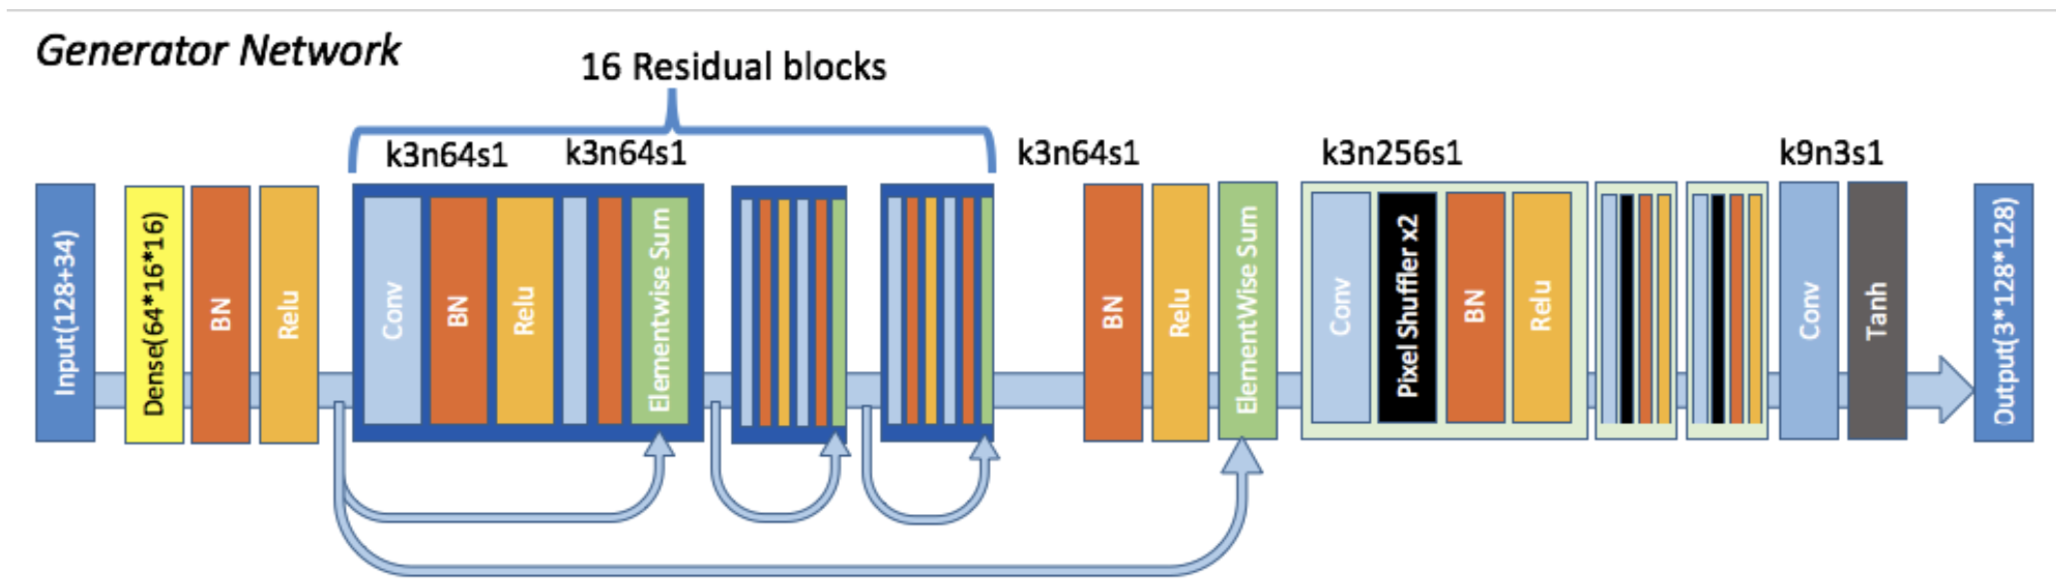
\includegraphics[width=1\linewidth]{figs/g_net_moe.png}
  \caption{\kai 生成网络。采用了16个Residual Block,降低了ReLU的出现频率,增加了横跨所有Residual Block的连接。图片来自于~\cite{Jin2017Towards}。}
  \label{fig:generator}
\end{figure}
\begin{figure}[H]
  \centering
  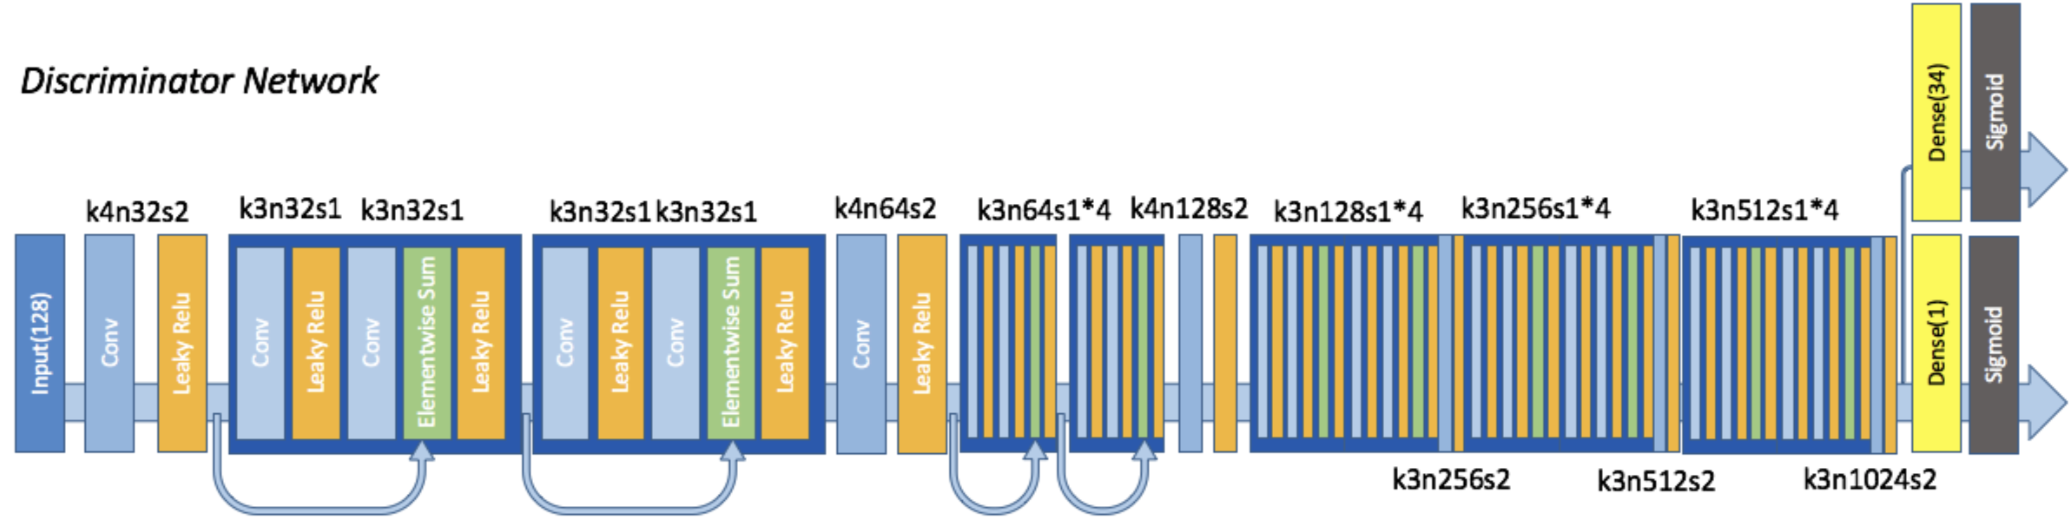
\includegraphics[width=1\linewidth]{figs/mod_disc.png}
  \caption{\kai 判别网络。采用了10个Residual Block,不使用Batch Normalization~\cite{ioffe2015batch}。图片来自于~\cite{Jin2017Towards}。}
  \label{fig:discriminator}
\end{figure}

我们在探究最佳训练的过程中还使用了Wassertein GAN~\cite{2017arXiv170107875A},其目标和损失函数定义如下:
%
\begin{align}
  \min_{\theta_G,\theta_f} \max_{\theta_D} \mathbb{E}_{(x, z, c) \sim (P_r, P_z, P_c)} \Big[ D(x) - D(G(z, c)) + \mathcal{L}_{gp} \Big] \\
  \mathcal{L}_{gp} = \norm{\left(\frac{\partial D(\tilde x)}{\partial \tilde x}\right)^2 - 1 }_2
\end{align}
%
其中$\tilde x$表示了生成图像和真实图像的线性插值,$\alpha \in (0, 1)$是随机的插值系数,即
%
\begin{equation}
  \tilde x = \alpha (x - G(z, c)) + G(z, c)
\end{equation}

为了扩展至第二阶段,我们加入了重建损失项。判别函数输入当前图像,除了输出一个真假判别项,还需要重建出 $z$ 和 $c$。生成器接受重建之后的$\hat z$和$\hat c$,生成重建图像$x_{rec}$,并加入关于重建图像的判别器损失和L1像素级别重建损失。同时为了增强判别器回归出$z$ 和 $c$的能力,还加入了判别器重建的损失,$z$由于是连续的,加入L1损失;$c$是离散的且含有类别信息,使用交叉熵作为损失。

\begin{align}
  \mathcal{L}_{IAN}(D) &= \mathcal{L}_{DRAGAN}(D) + \mathcal{L}_{reconstruct}(D) + \lambda_{adv} \mathcal{L}_{rec\_adv}(D)\\
  \mathcal{L}_{IAN}(G) &= \mathcal{L}_{DRAGAN}(G) + \mathcal{L}_{reconstruct}(G) + \lambda_{adv} \mathcal{L}_{rec\_adv}(G) \\
  \mathcal{L}_{reconstruct}(D) = \mathbb{E}_{x \sim P_{data}} \big[ \norm{x_{rec} - x} \big] + \mathbb{E}_{z\sim P_{noise},c\sim P_{cond}} \big[\norm{D_z(G(z, c)) - z} + P_D[c|D_c(G(z, c))] \big] \\
  \mathcal{L}_{reconstruct}(G) = \mathbb{E}_{x \sim P_{data}} \big[ \norm{x_{rec} - x} \big] + \mathbb{E}_{z\sim P_{noise},c\sim P_{cond}} \big[\norm{D_z(G(z, c)) - z} + P_D[c|D_c(G(z, c))] \big] \\
  \mathcal{L}_{rec\_adv}(D) = \mathbb{E}_{} \big[ log D(x_{rec}) \big] \\
  \mathcal{L}_{rec\_adv}(G) = \mathbb{E}_{} \big[ log (1 - D(x_{rec})) \big] \\
  x_{rec} = G(D_z(x), D_c(x))
\end{align}

扩展后的损失函数可用于第二阶段的工作,首先将真实图片经过判别器编码成z和c,然后使用生成器进行重建,就可以接入第一阶段的工作,完成重建。

\subsection{数据集}
我们使用的数据集取自 Getchu\footnote{\url{http://getchu.com}}网站,该网站汇聚了大量高质量动漫人物立绘,且图片中仅有单人,背景为白色,很适合作为我们的训练数据。

我们使用爬虫工具从该网站上获得了 22~000 张图片,经过 OpenCV \footnote{\url{https://opencv.org}}识别人脸,然后缩放、裁剪到 $64\times64$大小,并用 illustration2vec~\cite{Saito2015Illustration2Vec}对数据集进行了分类,具体类别如图~\ref{fig:getchu_cls}。根据类别可以得到 34 维的条件向量,如图~\ref{fig:ill_c}~所示。

\begin{figure}[H]
  \centering
  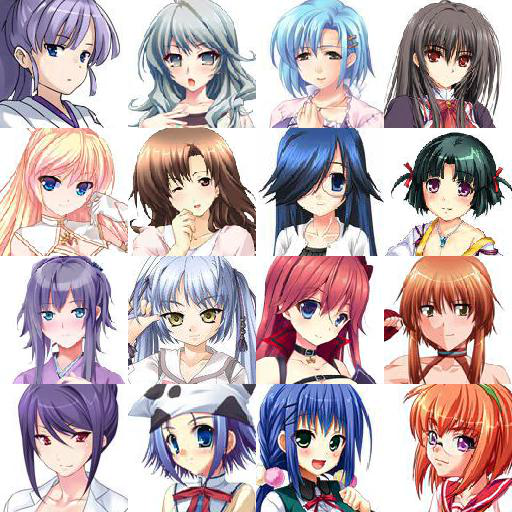
\includegraphics[width=0.5\linewidth]{figs/ex6.png}
  \caption{\kai Getchu数据集。采用opencv识别人脸,经过crop、scale到64x64的大小。}
  \label{fig:getchu_disp}
\end{figure}
\begin{figure}[H]
  \centering
  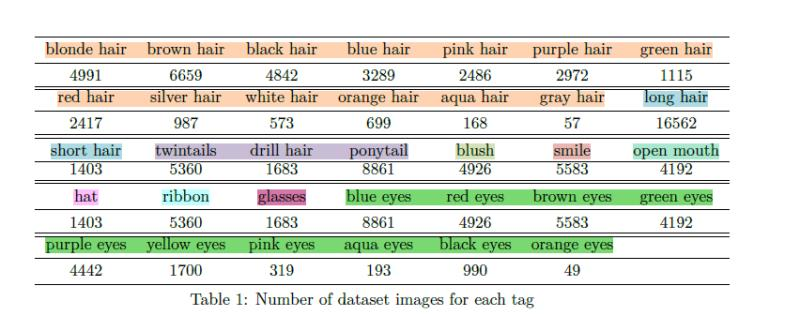
\includegraphics[width=0.8\linewidth]{figs/label_many.jpeg}
  \caption{\kai Getchu数据集分类详细描述。使用illustration2vec对数据集进行了分类,一共形成了34个类别。}
  \label{fig:getchu_cls}
\end{figure}
\begin{figure}[H]
  \centering
  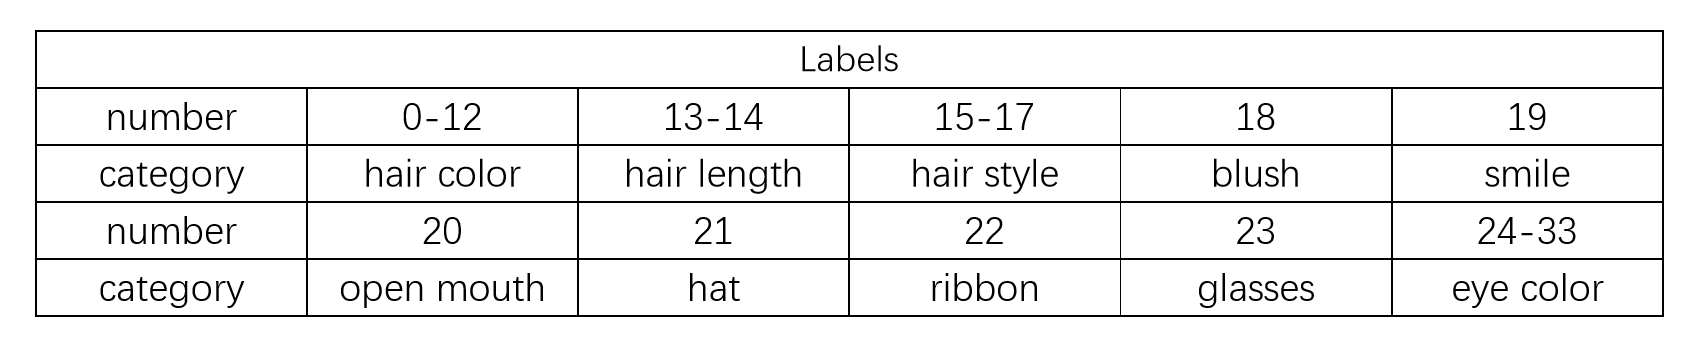
\includegraphics[width=0.8\linewidth]{figs/label_tiny.png}
  \caption{\kai 条件向量的构成。}
  \label{fig:ill_c}
\end{figure}

\section{实验}
\subsection{生成对抗训练}

在我们完成项目的过程中,在MNIST数据集和自定义的Getchu数据集上都进行了多次实验,包括网络结构的选取、训练参数的设置,普通GAN训练、WGAN~\cite{2017arXiv170107875A}和DRAGAN等训练方法的选取。

\subsubsection{演示模型的训练}

最终我们确定的训练设置是:Adam~\cite{Kingma2014Adam}优化器以$2 \times 10^{-4}$的初始学习率进行$5 \times 10^{4}$的迭代,然后在接下来$5 \times 10^{4}$的迭代中线性降低学习率至$1 \times 10^{5}$。网络使用128维的随机向量$z$和34维的条件向量$c$,前者服从$\sigma=1, \mu=0$的正态分布,后者在保证类互斥条件下由均匀分布随机产生。各个loss的系数是$\lambda_{gp}=0.5$,$\lambda_{reg}=10^{-4}$,$\lambda_{adv}=1$。$\mathrm{batchsize}=64$。训练在Titan X GPU下需要花费大约20小时的时间。

图~\ref{fig:goodmodel_dragan}~展示了我们使用的演示模型的训练loss变化:

\begin{figure}[H]
  \centering
  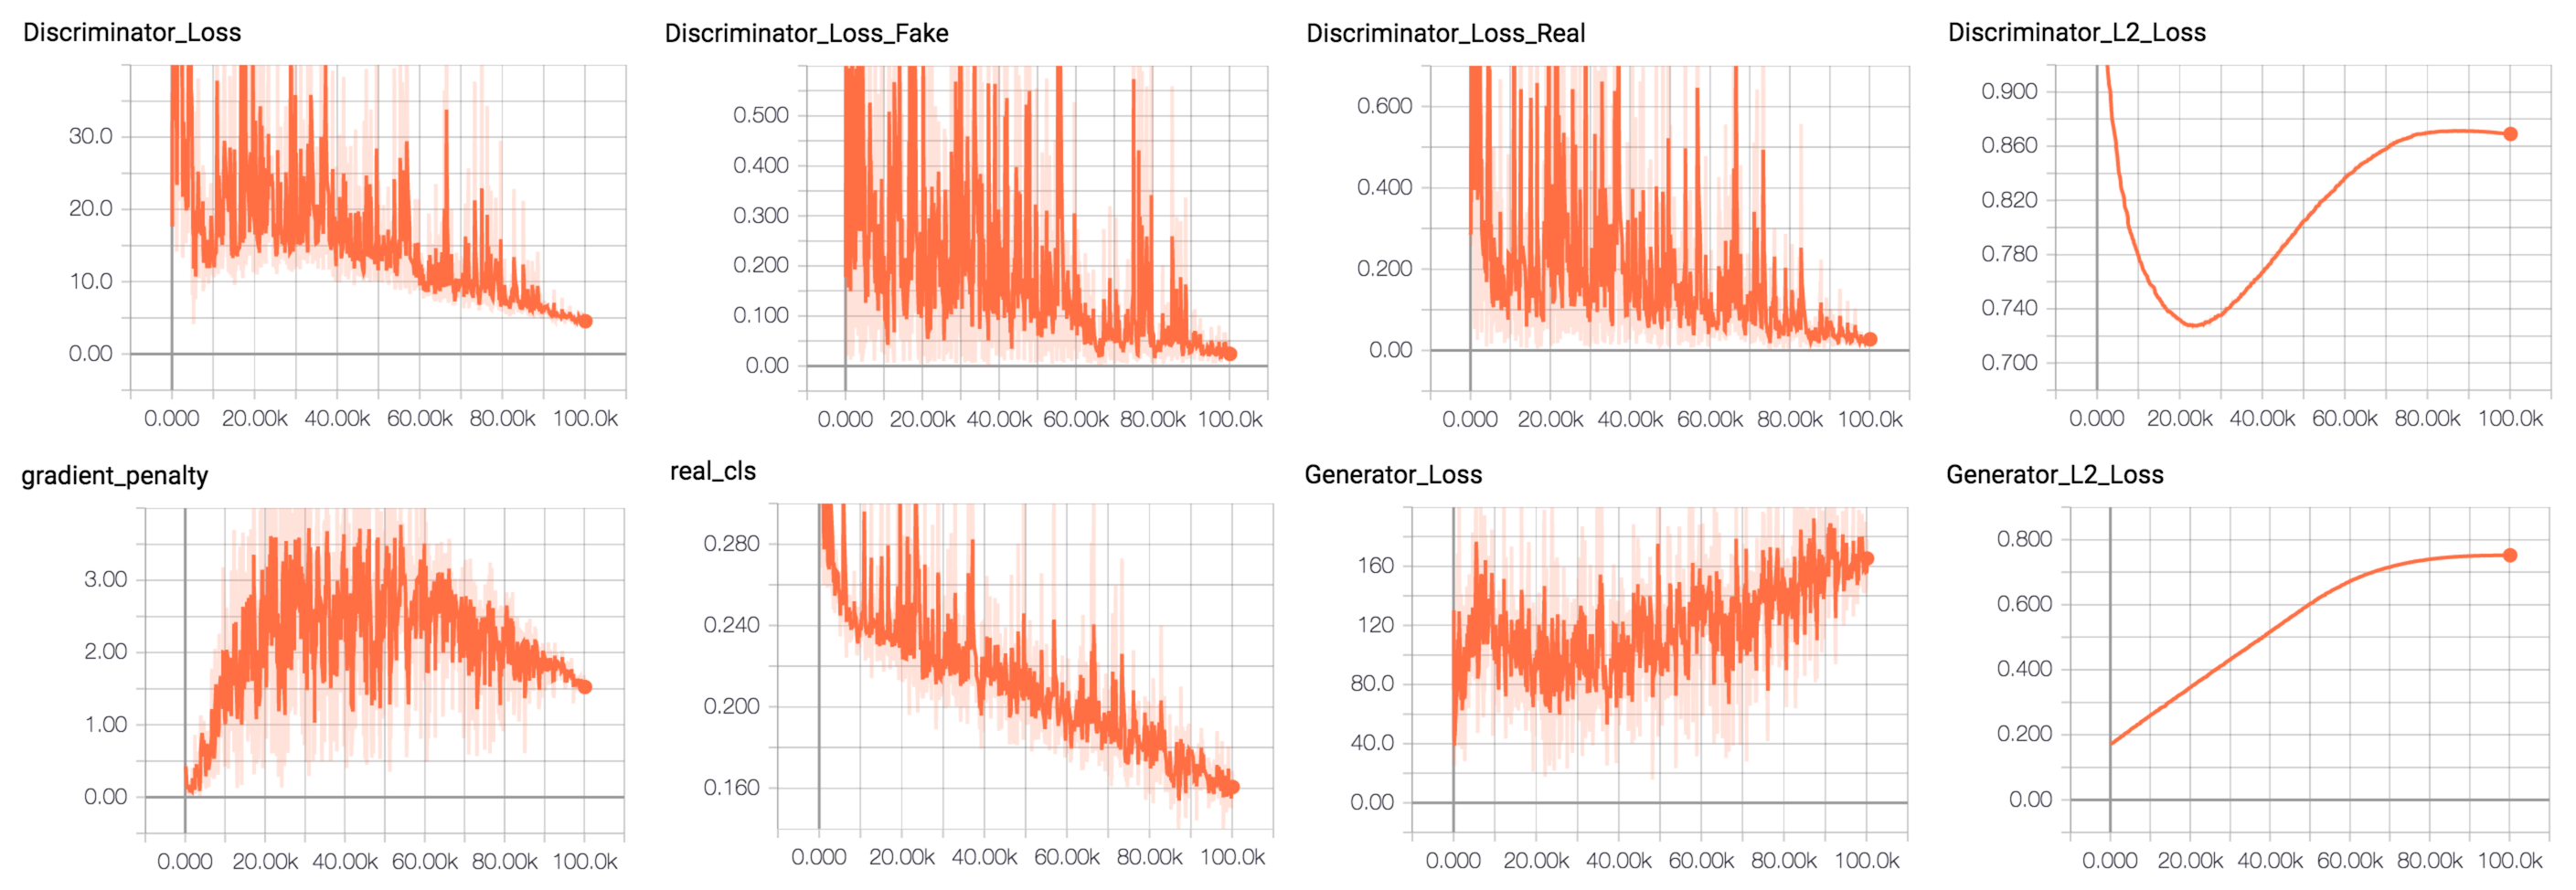
\includegraphics[width=1\linewidth]{figs/good_model_dragan.png}
  \caption{\kai 演示模型的训练loss图。左上角开始的Discriminator Loss是判别器的总损失,其右的Fake和Real损失分别是判别器识别生成图片和真实图片的损失。左下角的gradient penalty如上文所述,其右是判别器分类图片的交叉熵损失。再右边是Generator Loss的总损失,最右边是两个网络的正则损失。}
  \label{fig:goodmodel_dragan}
\end{figure}

可以看出生成器的损失除了刚刚开始的震荡较为剧烈以外,整体在稳步下降。查看固定随机数的生成结果,如图~\ref{fig:dragan_evolve}~所示。从每一个随机种子生成的图片可以看到生成的不断完善、生成结果质量的稳定上升。

\begin{figure}[H]
  \centering
  \includegraphics[width=1\linewidth]{figs/good_model_dragan_sample.png}
  \caption{\kai 演示模型的训练中生成图像的演化。从左到右四张图片分别是25k, 50k, 75k, 100k迭代时的生成结果。每一张图片包含16个固定随机数生成的结果。}
  \label{fig:dragan_evolve}
\end{figure}

\subsubsection{参数调节实验}

此处展示的是探究WGAN中$\lambda_{adv}$比例的实验。与演示模型的训练不同,此时我们使用的是Wassertain GAN而不是DRAGAN,在训练的初期不稳定而在中后期十分稳定。训练的学习率从$1 \times 10^{-4}$开始,经过$1 \times 10^{5}$的迭代后学习率开始线性下降,经过$1 \times 10^{5}$的迭代降到$1 \times 10^{-5}$。

\begin{figure}[H]
  \centering
  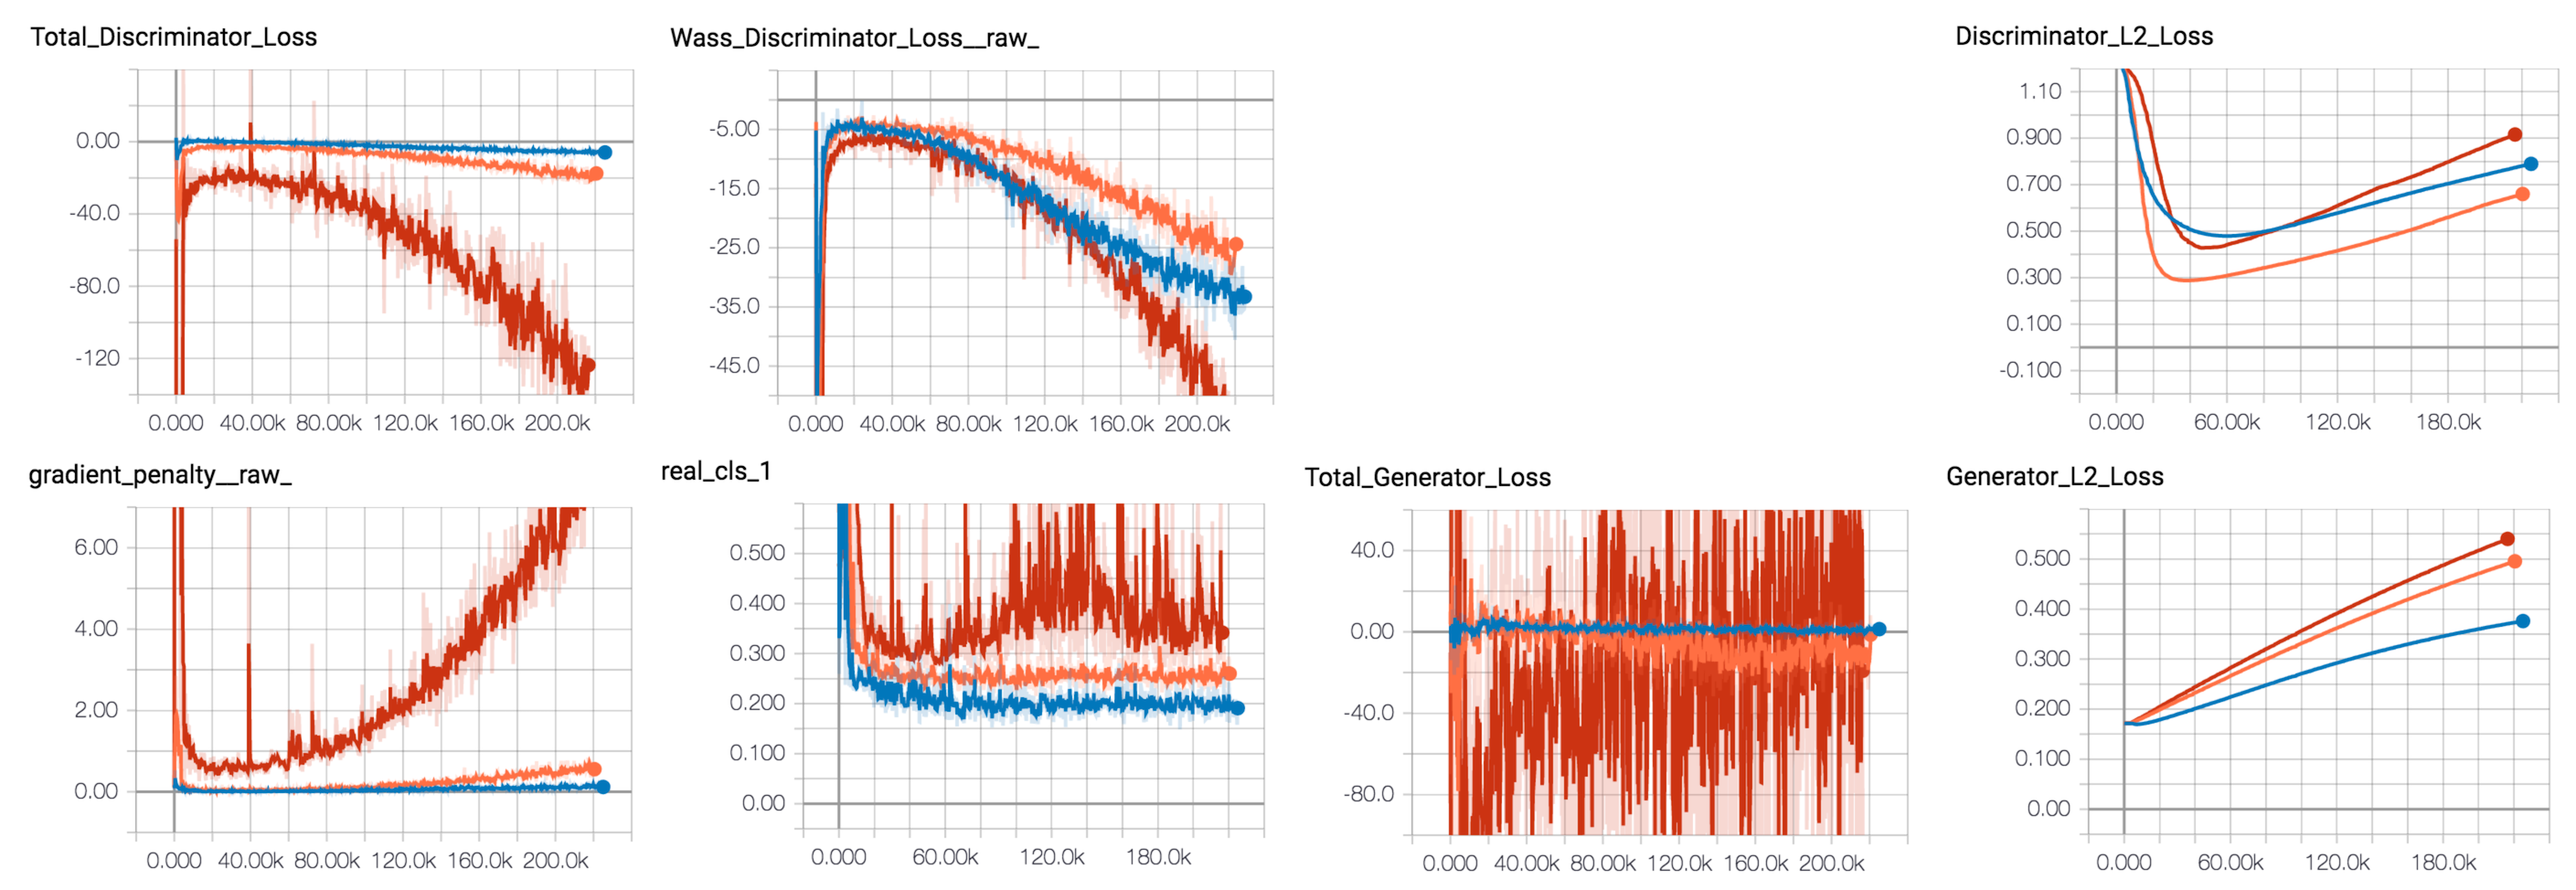
\includegraphics[width=1\linewidth]{figs/good_model_wgan.png}
  \caption{\kai WGAN中$\lambda_{adv}$调节实验。实验中橘色、蓝色、红色分别对应了$\lambda_{adv}=0.25, 1, 4$的情况。左上角的是判别器的总损失,其右是没有经过系数缩放的Wassertain损失。由于Wassertain GAN的特性,没有明确区分的fake和real判别损失,故其右边一格是空图。左下角依次是gradient penalty,判别器分类损失,生成器总损失。最右边一列是两个网络的正则化。}
  \label{fig:goodmodel_wgan}
\end{figure}

训练过程中loss的变化如图~\ref{fig:goodmodel_wgan}~所示。我们发现WGAN的判别器loss呈现抛物线的形状,在前中期不断上升,在后期开始一路下滑。在众多WGAN的文献中WGAN普遍呈现初期是较大的负数,之后稳定上升的情况,没有关于先升后降应当如何解释的记载。

判别器损失越趋向于负数,则其判别出生成图像的能力越强,虽然无法推断后期的下降是由什么引起,但是从生成结果图~\ref{fig:wgan_evolve}~中并没有看出明显的质量下降,网络没有出现训练崩溃的情况。

\begin{figure}[H]
  \centering
  \includegraphics[width=1\linewidth]{figs/good_model_wgan_sample.png}
  \caption{\kai Wassertain GAN参数调节实验中生成图像的演化。每一张图片包含16个固定随机数生成的结果。三行由上至下是$\lambda_{adv}=0.25, 1, 4$的情况,从左到右是18k, 92k, 182k迭代时生成的结果,对应于WGAN训练过程中的初期、中期、后期。初期到中期体现出生成质量上升,中期到后期质量略有下降。$\lambda_{adv}=1$时质量最好。}
  \label{fig:wgan_evolve}
\end{figure}

最终我们确定了WGAN使用$\lambda_{adv}=1$作为WGAN训练的设置。然而与DRAGAN的训练结果相比,WGAN的生成质量略有不如,最终选用DRAGAN作为网络训练的方法。

\subsubsection{MNIST的IAN训练}

使用上文中的IAN损失,我们成功训练了带AutoEncoder功能的判别器。从~\ref{fig:mnist_ian}中可以看出生成数字和重建数字的演变。生成的质量在稳步提升,数字的比划变得越来越清晰。值得注意的是重建数字在较早的时刻已经能够完成正确类别的重建,证明判别器学习c的重建快于重建z的学习,也证明生成器较早低学习到了c表示类别的能力。

然而具体数字的形状在训练较为晚期的时候依然没能有准确的重建,可能是由于使用L1损失函数作为z重建的损失函数并不合适,也可能是由于损失函数之间系数不平衡,需要后续研究进行确认。

\begin{figure}[H]
  \centering
  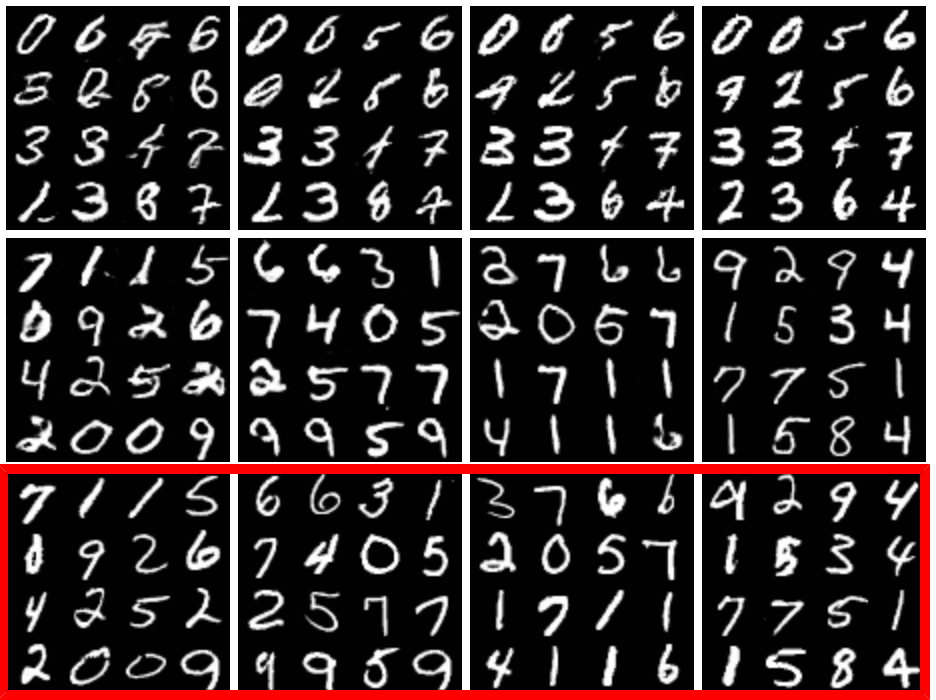
\includegraphics[width=1\linewidth]{figs/mnist.png}
  \caption{\kai NNIST上的IAN训练。由上至下第一行是固定z和c生成的结果,第二行是重建的结果,第三行红框之中的是用于重建的原图。从左至右是25k, 50k, 100k, 200k迭代时候的结果,生成质量和重建质量的提升十分明显。}
  \label{fig:mnist_ian}
\end{figure}


\subsection{图像编辑}

\subsubsection{实际设置}

在实际测试中,我们经过测试,最终选择了使用DRAGAN训练的模型进行图像编辑。

同时,我们对$z$和$c$选择了不同的学习率。经过调试,我们将$z$的学习率设置为$0.20$,$c$的学习率设置为$0.10$。我们在原先将学习率在函数中定义为常数,修改较为麻烦,后来为了方便调试,我们将学习率的获取方式修改为从文件中读取,这样可以在不关闭前端的情况下修改学习率进行调试,大大加快了调试速度,最终获得了效果较为优秀的参数。

我们原先的想法是直接对于$z$和$c$在原函数域上进行训练,但经过推导,我们认为这样的训练并不符合$z$和$c$的分布,因此训练效果较差。因此我们最终选择对于$z$在$\tanh$函数的反函数域上的对应值$\tilde z$和$c$在 sigmoid 函数的反函数域上的对应值$\tilde c$进行训练。经过这样的修改,我们取得了较好的的训练效果。

为了使$z$和$c$在修改后仍然有意义,我们对于$z$和$c$在反函数域上的对应值$\tilde z$和$\tilde c$进行了边界限制,将$\tilde z$和$\tilde c$的取值范围限制在$(-10.0, 10.0)$之间,避免不合法的参数出现。同时,因为$c$是由多个代表不同人物特征,如发色、瞳色等的one-hot向量连接成的向量,我们对于由经过训练后的$\tilde c'$生成的$c'$向量也进行了类似的处理,让$c'$在每个对应的部分为one-hot向量,以保证数据合法性。

\subsubsection{效果展示}

<<<<<<< HEAD
将编辑操作应用于训练好的网络,我们得到了效果优秀的图像生成和编辑效果。我们的模型我们的模型能够生成高质量的图片,并对其进行稳定的编辑,在编辑过程中不容易丧失图片的真实性。同时编辑支持多种功能,眼睛、头发的颜色,发型等可以按照简笔画给定的方式变化。

在图~\ref{fig:pic}中,第一行的两组为更换发色的例子,第二行的两组为更换瞳色的例子,第三行的两组为更换发型的例子。可以看出,第一行中,左边的一组成功将原图中的人物的发色从白色变成了红色,而右边的一组成功将原图中的人物的发色从红色变成了黑色。第二行中,左边的一组成功将人物瞳色从红色变成了蓝色,而右边的一组将人物瞳色从蓝色变成了紫红色。第三行中,左边的一组成功在人物头上添加了一束紫色的头发,而右边的一组成功去掉了人物头两侧的头发,将人物从长发变成了短发。
=======
将编辑操作应用于训练好的网络,我们得到了效果优秀的图像生成和编辑效果。如图~\ref{fig:pic}~所示,我们的模型我们的模型能够生成高质量的图片,并对其进行稳定的编辑,在编辑过程中不容易丧失图片的真实性。同时编辑支持多种功能,眼睛、头发的颜色,发型等可以按照简笔画给定的方式变化。

\begin{figure}[H]
  \centering
  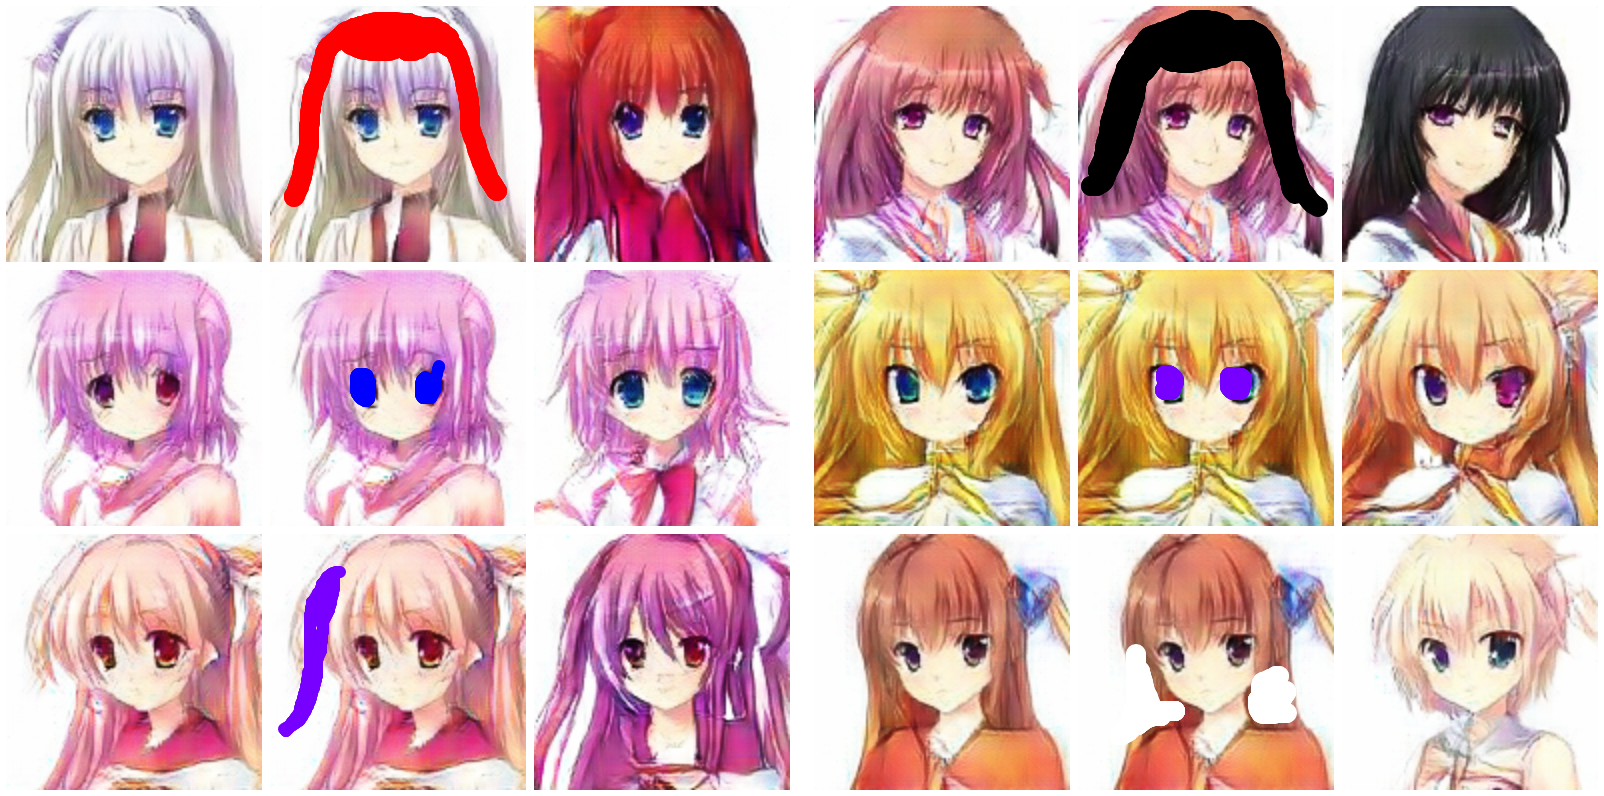
\includegraphics[width=0.9\linewidth]{figs/pic.png}
  \caption{\kai 编辑效果展示,共六组,每组三幅图。每组中最左边的一幅为原图,中间的一幅图为编辑图,最右边的一幅图为生成的结果图。第一行为成功更换发色的例子,第二行为成功更换瞳色的例子,第三行为成功更换发型的例子。}
  \label{fig:pic}
\end{figure}

在图~\ref{fig:pic}~中,第一行的两组为更换发色的例子,第二行的两组为更换瞳色的例子,第三行的两组为更换发型的例子。可以看出,第一行中,左边的一组成功将原图中的人物的发色从白色变成了红色,而右边的一组成功将原图中的人物的发色从红色变成了黑色。第二行中,左边的一组成功将人物瞳色从红色变成了蓝色,而右边的一组将人物瞳色从蓝色变成了紫红色。第三行中,左边的一组成功在人物头上添加了一束紫色的头发,而右边的一组成功去掉了人物头两侧的头发,将人物从长发变成了短发。
>>>>>>> 082ba19c572184d19d7188546e3b9b3ad1bff49d

可以看出,我们生成的模型可以进行对动漫人物的发色、瞳色、发型等多方面特征进行编辑,且效果出色。与基线相比,生成质量上升,生成清晰度上升,编辑稳定性提高,编辑多样性也有提高。

\subsection{网页应用}

我们基于训练好的模型,构建了一个基于 B/S 架构的网页应用,可以通过 Web 浏览器进行在线图像编辑。

\subsubsection{网页端}
我们的网页端界面如图 \ref{figure:web1} $\sim$ 图 \ref{figure:web3}  所示,能够运行在任何一款现代浏览器上。

\begin{figure}[H]
  \begin{minipage}[t]{0.33\linewidth}
      \centering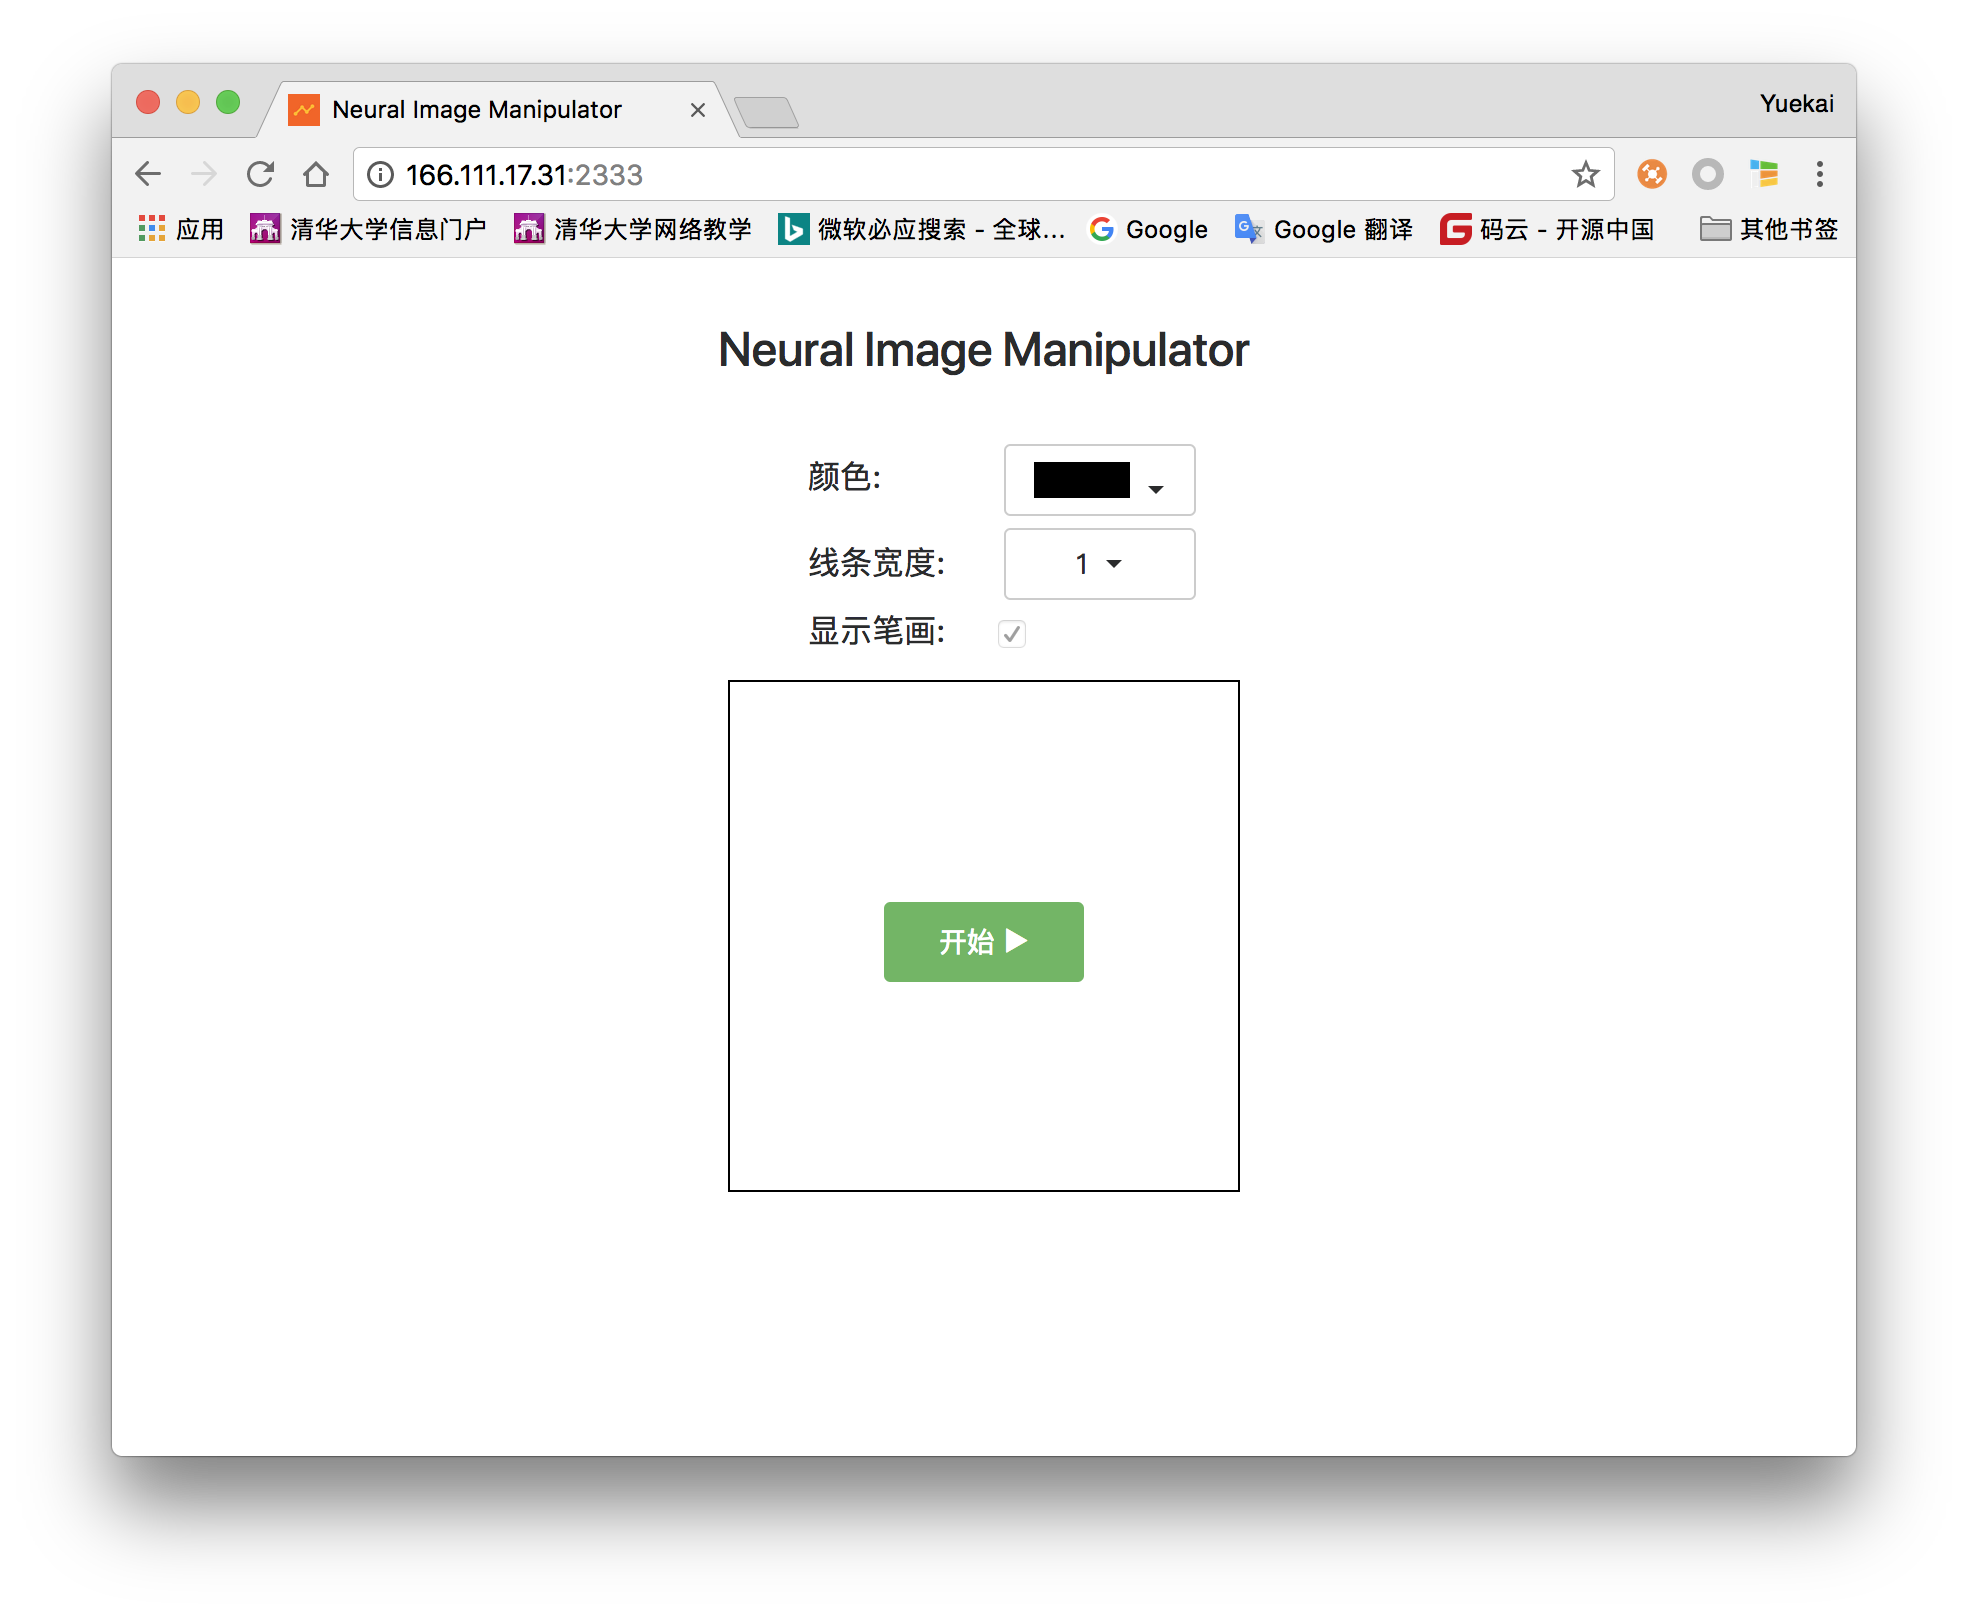
\includegraphics[height=4cm]{figs/web1.png}
      \caption{\kai 开始页面}\label{figure:web1}
  \end{minipage}%
  \begin{minipage}[t]{0.33\linewidth}
      \centering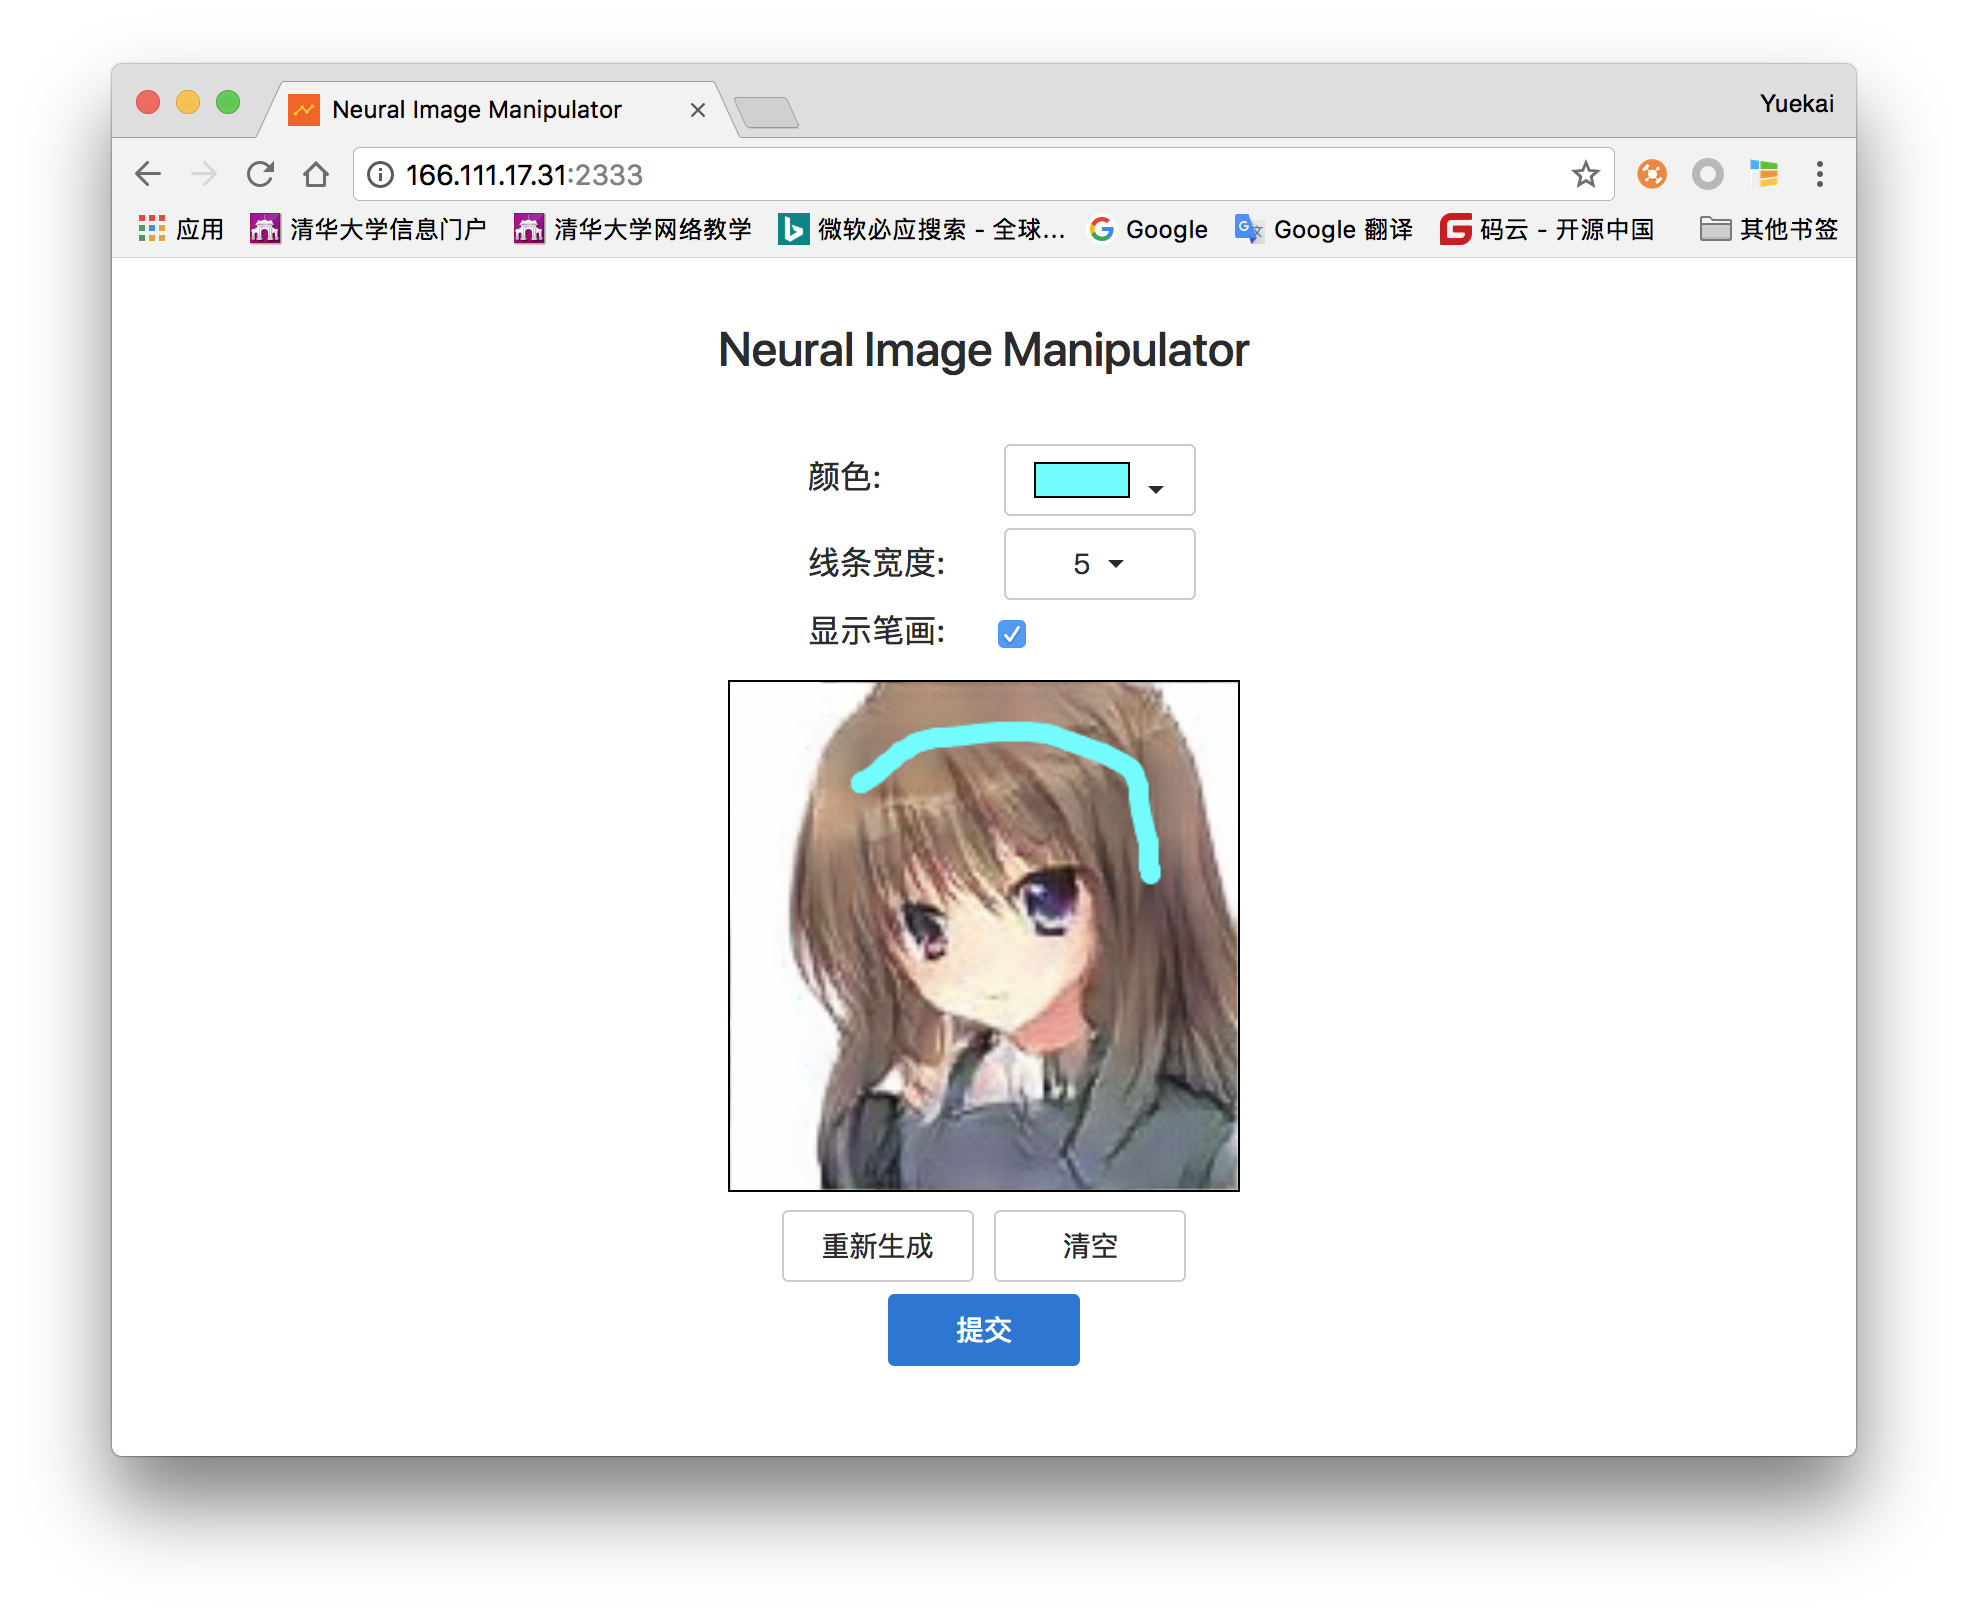
\includegraphics[height=4cm]{figs/web2.png}
      \caption{\kai 输入笔画}\label{figure:web2}
  \end{minipage}%
  \begin{minipage}[t]{0.33\linewidth}
      \centering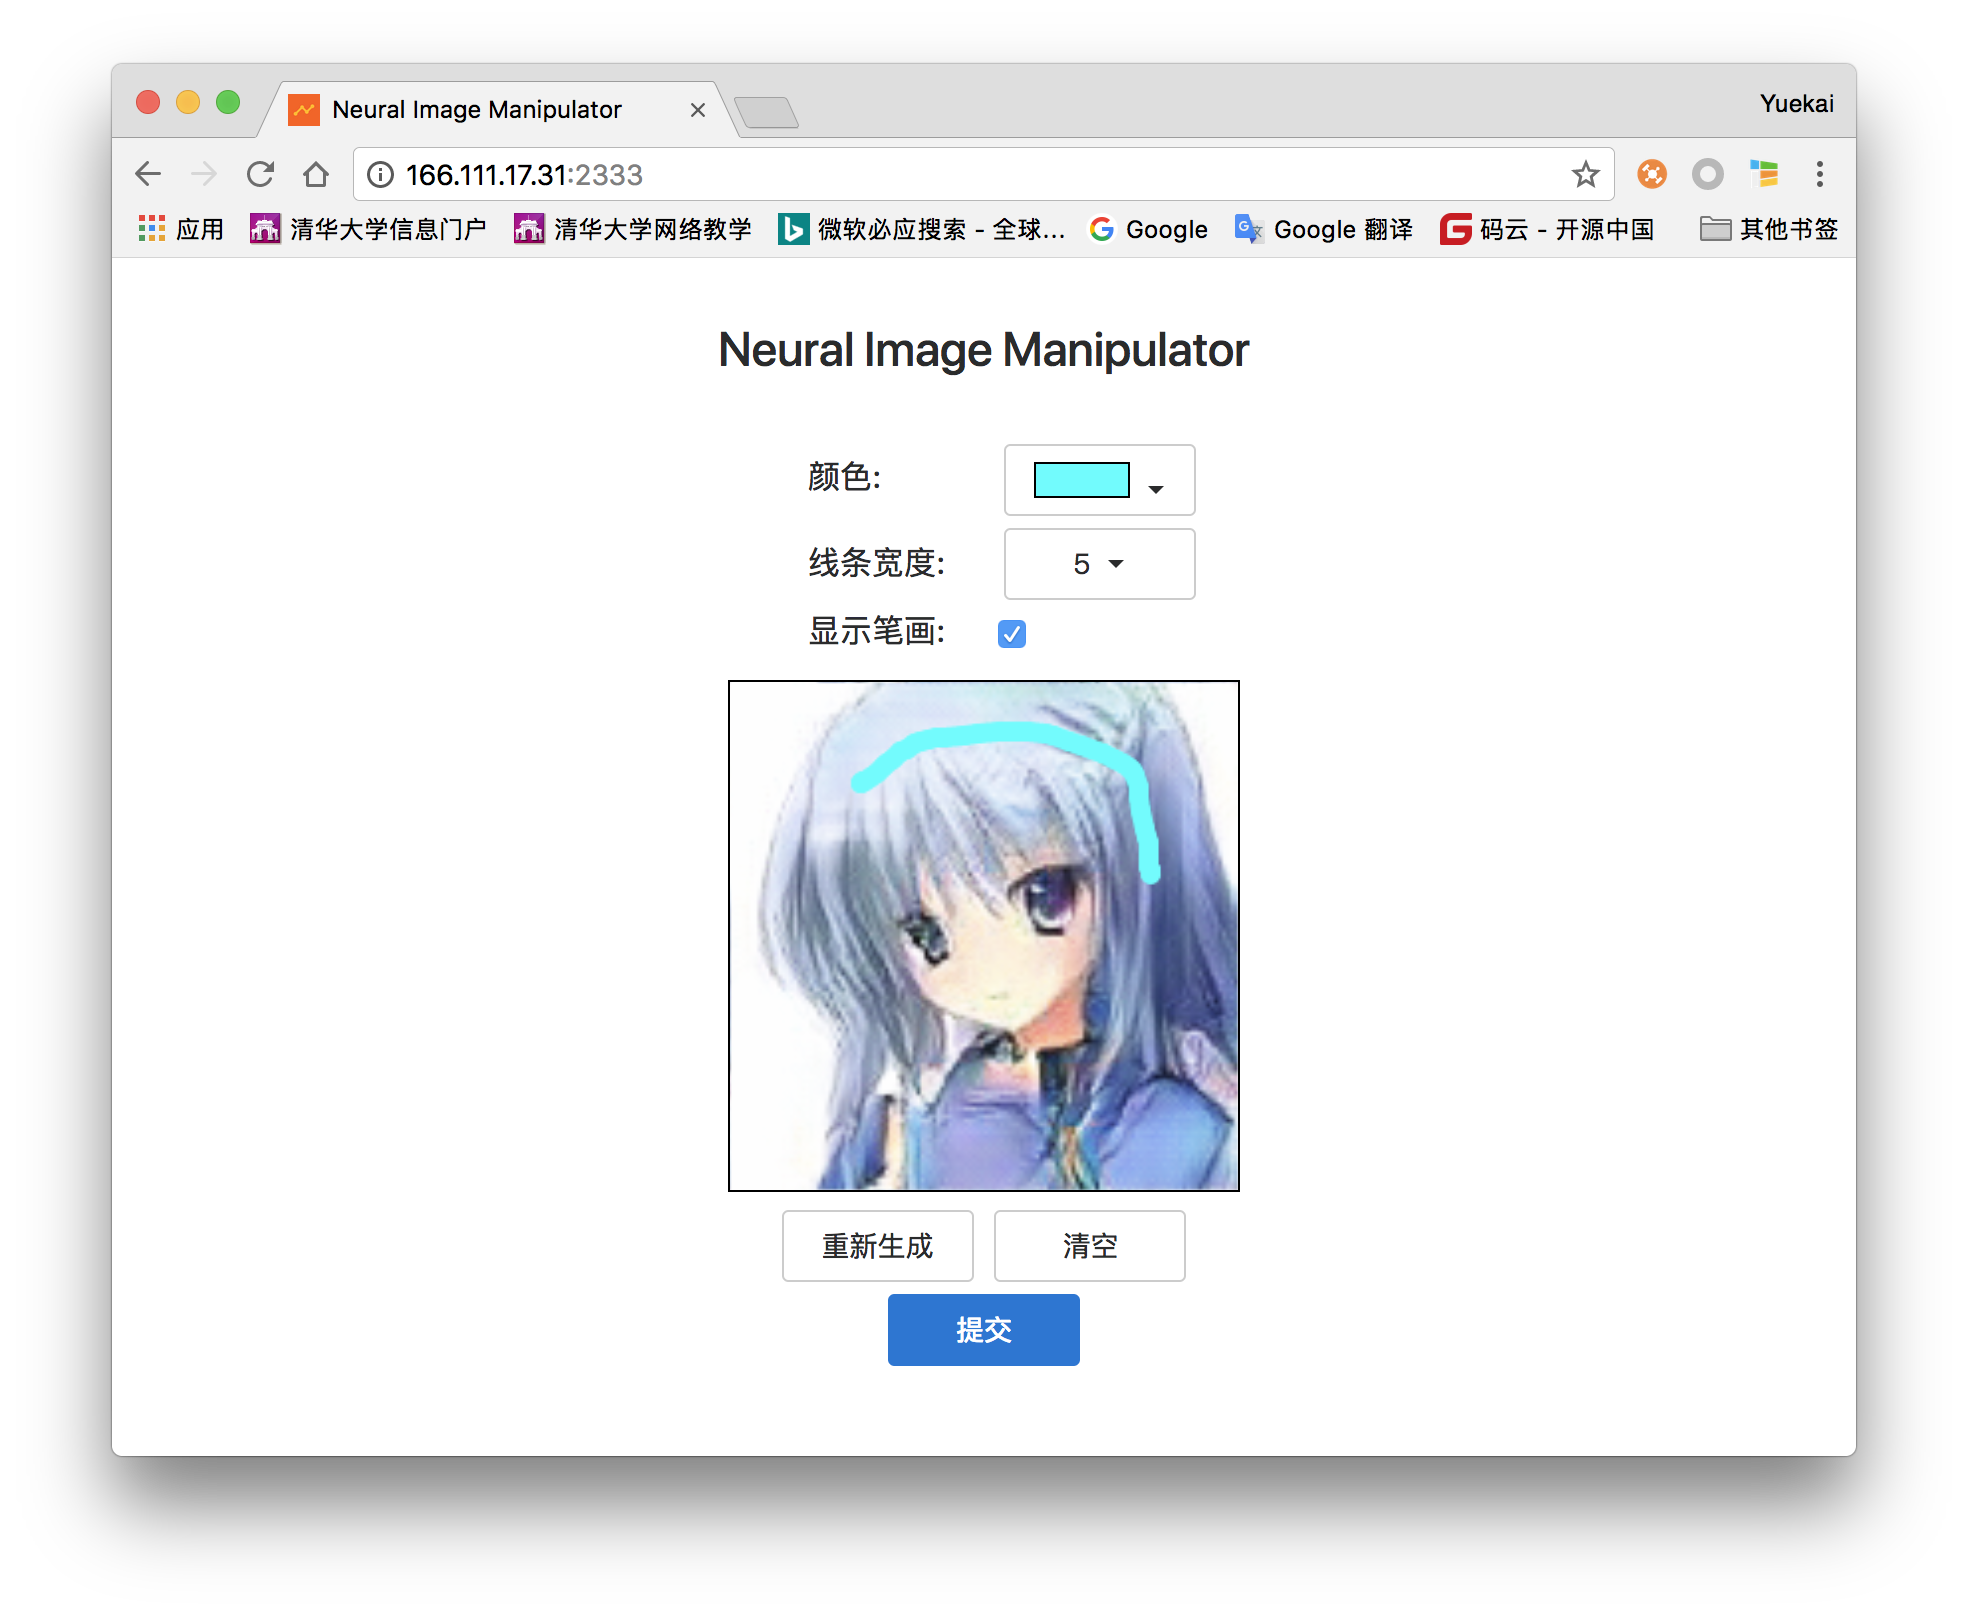
\includegraphics[height=4cm]{figs/web3.png}
      \caption{\kai 点击提交后}\label{figure:web3}
  \end{minipage}
\end{figure}

首次打开网页,点击 “开始按钮”,服务器会返回一张初始生成的图像。之后用户可以使用画笔工具,简单地勾勒出图片期望的变化方向,点击“提交”后,服务器就会返回在原图基础上,加上用户编辑条件后生成的图像;点击“重新生成”后,服务器会重新生成一张图片;点击“清空”能清空用户画的所有的笔画。此外,网页还支持更改画笔颜色、粗细,并能切换笔画的显示,以方便用户编辑。

该网页主要用 HTML 和 JavaScript 实现,并使用了 jQurey\footnote{\url{http://jquery.com}} 和 Bootstrap \footnote{\url{http://getbootstrap.com}} 等库。图片编辑框使用了 HTML5 的 \texttt{<canvas>},点击提交后,会将编辑框中的笔画图转成 Base64\footnote{\url{https://en.wikipedia.org/wiki/Base64}} 编码,使用 HTTP 请求发给服务器,之后服务器会返回生成图像的 Base64 编码,前端再将其作为图片编辑框的背景,显示给用户。

需要注意的是,用户每次点提交时,服务器是在该用户当前图像的基础上,再根据用户提供的笔画生成新图像,而且需要支持多用户同时编辑,即需要知道该用户当前的编辑状态。我们的做法是,服务器生成图像给前端时,会附带此时的 $z$ 和 $c$ 向量。前端将其保存下来,下次点提交时再发给服务器,服务器就会根据前端提供的 $z$ 和 $c$ 生成图像,以达到保存用户编辑状态的效果。

\subsubsection{服务器端}
由于训练模型使用的是 Python,所以我们选择了基于 Python 的 Django 框架搭建服务器端。

服务器端接收前端发来的笔画图,计算出 sketch 和 mask 矩阵,再根据前端发来的 $z$ 和 $c$,放入之前训练好的网络中,就能得到生成的图像。然后将其和修改后的 $z$ 和 $c$ 返回给前端。

实际测试时,模型的运行效率非常快,生成一张图像的时间仅需十几毫秒,主要延时在于网络传输。因此,就算是多个用户同时访问网页进行编辑,服务器也完全可以承受住这样的负载。

\section{结论}

本项目完成了神经图像编辑在动漫人脸数据集上的应用。我们尝试了多种模型与训练方法,找到了最佳的模型结构与参数,并实现了一个网页前端用于交互用户的编辑操作。与baseline方法相比较,我们的方法取得了如下的提升与贡献:

\begin{enumerate}
\item 成功复现了高质量的动漫人物头像生成网络。
\item 成功应用编辑图像方法于极深层的神经网络。
\item 获得了高于基线的生成成果和编辑成果。包括生成真实度上升,生成清晰度上升($64 \times 64 \Rightarrow 128 \times 128$)和肉眼可见的编辑质量上升
\item 基于Web/Server的交互界面。
\end{enumerate}

\section{个人收获}

寇明阳:通过这次的大作业,我理解了诸如WGAN、DCGAN等生成式对抗网络的模型和工作方法,了解并实现了使用GAN进行图像编辑的工作流程,也学习了一些读取网络模型、调试网络参数和处理数据的方法。在团队合作的过程中,我从同组同学的身上学习到了许多新的知识,有了很大的收获。
% -- 个人收获 ---【寇明扬】 【贾越凯】

\section*{参考文献}

\medskip

{\small
\bibliographystyle{ieee}
\bibliography{egbib}
}

\end{document}
